\documentclass{report}

%%%%%%%%%%%%%%%%%%%%%%%%%%%%%%%%%
% PACKAGE IMPORTS
%%%%%%%%%%%%%%%%%%%%%%%%%%%%%%%%%


\usepackage[tmargin=2cm,rmargin=1in,lmargin=1in,margin=0.85in,bmargin=2cm,footskip=.2in]{geometry}
\usepackage{amsmath,amsfonts,amsthm,amssymb,mathtools}
\usepackage[varbb]{newpxmath}
\usepackage{xfrac}
\usepackage[makeroom]{cancel}
\usepackage{mathtools}
\usepackage{bookmark}
\usepackage{enumitem}
\usepackage{hyperref,theoremref}
\hypersetup{
	pdftitle={Assignment},
	colorlinks=true, linkcolor=doc!90,
	bookmarksnumbered=true,
	bookmarksopen=true
}
\usepackage[most,many,breakable]{tcolorbox}
\usepackage{xcolor}
\usepackage{varwidth}
\usepackage{varwidth}
\usepackage{etoolbox}
%\usepackage{authblk}
\usepackage{nameref}
\usepackage{multicol,array}
\usepackage{tikz-cd}
\usepackage[ruled,vlined,linesnumbered]{algorithm2e}
\usepackage{comment} % enables the use of multi-line comments (\ifx \fi) 
\usepackage{import}
\usepackage{xifthen}
\usepackage{pdfpages}
\usepackage{transparent}

\newcommand\mycommfont[1]{\footnotesize\ttfamily\textcolor{blue}{#1}}
\SetCommentSty{mycommfont}
\newcommand{\incfig}[1]{%
    \def\svgwidth{\columnwidth}
    \import{./figures/}{#1.pdf_tex}
}

\usepackage{tikzsymbols}
\renewcommand\qedsymbol{$\Laughey$}


%\usepackage{import}
%\usepackage{xifthen}
%\usepackage{pdfpages}
%\usepackage{transparent}


%%%%%%%%%%%%%%%%%%%%%%%%%%%%%%
% SELF MADE COLORS
%%%%%%%%%%%%%%%%%%%%%%%%%%%%%%



\definecolor{myg}{RGB}{56, 140, 70}
\definecolor{myb}{RGB}{45, 111, 177}
\definecolor{myr}{RGB}{199, 68, 64}
\definecolor{mytheorembg}{HTML}{F2F2F9}
\definecolor{mytheoremfr}{HTML}{00007B}
\definecolor{mylenmabg}{HTML}{FFFAF8}
\definecolor{mylenmafr}{HTML}{983b0f}
\definecolor{mypropbg}{HTML}{f2fbfc}
\definecolor{mypropfr}{HTML}{191971}
\definecolor{myexamplebg}{HTML}{F2FBF8}
\definecolor{myexamplefr}{HTML}{88D6D1}
\definecolor{myexampleti}{HTML}{2A7F7F}
\definecolor{mydefinitbg}{HTML}{E5E5FF}
\definecolor{mydefinitfr}{HTML}{3F3FA3}
\definecolor{notesgreen}{RGB}{0,162,0}
\definecolor{myp}{RGB}{197, 92, 212}
\definecolor{mygr}{HTML}{2C3338}
\definecolor{myred}{RGB}{127,0,0}
\definecolor{myyellow}{RGB}{169,121,69}
\definecolor{myexercisebg}{HTML}{F2FBF8}
\definecolor{myexercisefg}{HTML}{88D6D1}


%%%%%%%%%%%%%%%%%%%%%%%%%%%%
% TCOLORBOX SETUPS
%%%%%%%%%%%%%%%%%%%%%%%%%%%%

\setlength{\parindent}{1cm}
%================================
% THEOREM BOX
%================================

\tcbuselibrary{theorems,skins,hooks}
\newtcbtheorem[number within=section]{Theorem}{Theorem}
{%
	enhanced,
	breakable,
	colback = mytheorembg,
	frame hidden,
	boxrule = 0sp,
	borderline west = {2pt}{0pt}{mytheoremfr},
	sharp corners,
	detach title,
	before upper = \tcbtitle\par\smallskip,
	coltitle = mytheoremfr,
	fonttitle = \bfseries\sffamily,
	description font = \mdseries,
	separator sign none,
	segmentation style={solid, mytheoremfr},
}
{th}

\tcbuselibrary{theorems,skins,hooks}
\newtcbtheorem[number within=chapter]{theorem}{Theorem}
{%
	enhanced,
	breakable,
	colback = mytheorembg,
	frame hidden,
	boxrule = 0sp,
	borderline west = {2pt}{0pt}{mytheoremfr},
	sharp corners,
	detach title,
	before upper = \tcbtitle\par\smallskip,
	coltitle = mytheoremfr,
	fonttitle = \bfseries\sffamily,
	description font = \mdseries,
	separator sign none,
	segmentation style={solid, mytheoremfr},
}
{th}


\tcbuselibrary{theorems,skins,hooks}
\newtcolorbox{Theoremcon}
{%
	enhanced
	,breakable
	,colback = mytheorembg
	,frame hidden
	,boxrule = 0sp
	,borderline west = {2pt}{0pt}{mytheoremfr}
	,sharp corners
	,description font = \mdseries
	,separator sign none
}

%================================
% Corollery
%================================
\tcbuselibrary{theorems,skins,hooks}
\newtcbtheorem[number within=section]{Corollary}{Corollary}
{%
	enhanced
	,breakable
	,colback = myp!10
	,frame hidden
	,boxrule = 0sp
	,borderline west = {2pt}{0pt}{myp!85!black}
	,sharp corners
	,detach title
	,before upper = \tcbtitle\par\smallskip
	,coltitle = myp!85!black
	,fonttitle = \bfseries\sffamily
	,description font = \mdseries
	,separator sign none
	,segmentation style={solid, myp!85!black}
}
{th}
\tcbuselibrary{theorems,skins,hooks}
\newtcbtheorem[number within=chapter]{corollary}{Corollary}
{%
	enhanced
	,breakable
	,colback = myp!10
	,frame hidden
	,boxrule = 0sp
	,borderline west = {2pt}{0pt}{myp!85!black}
	,sharp corners
	,detach title
	,before upper = \tcbtitle\par\smallskip
	,coltitle = myp!85!black
	,fonttitle = \bfseries\sffamily
	,description font = \mdseries
	,separator sign none
	,segmentation style={solid, myp!85!black}
}
{th}


%================================
% LENMA
%================================

\tcbuselibrary{theorems,skins,hooks}
\newtcbtheorem[number within=section]{Lenma}{Lenma}
{%
	enhanced,
	breakable,
	colback = mylenmabg,
	frame hidden,
	boxrule = 0sp,
	borderline west = {2pt}{0pt}{mylenmafr},
	sharp corners,
	detach title,
	before upper = \tcbtitle\par\smallskip,
	coltitle = mylenmafr,
	fonttitle = \bfseries\sffamily,
	description font = \mdseries,
	separator sign none,
	segmentation style={solid, mylenmafr},
}
{th}

\tcbuselibrary{theorems,skins,hooks}
\newtcbtheorem[number within=chapter]{lenma}{Lenma}
{%
	enhanced,
	breakable,
	colback = mylenmabg,
	frame hidden,
	boxrule = 0sp,
	borderline west = {2pt}{0pt}{mylenmafr},
	sharp corners,
	detach title,
	before upper = \tcbtitle\par\smallskip,
	coltitle = mylenmafr,
	fonttitle = \bfseries\sffamily,
	description font = \mdseries,
	separator sign none,
	segmentation style={solid, mylenmafr},
}
{th}


%================================
% PROPOSITION
%================================

\tcbuselibrary{theorems,skins,hooks}
\newtcbtheorem[number within=section]{Prop}{Proposition}
{%
	enhanced,
	breakable,
	colback = mypropbg,
	frame hidden,
	boxrule = 0sp,
	borderline west = {2pt}{0pt}{mypropfr},
	sharp corners,
	detach title,
	before upper = \tcbtitle\par\smallskip,
	coltitle = mypropfr,
	fonttitle = \bfseries\sffamily,
	description font = \mdseries,
	separator sign none,
	segmentation style={solid, mypropfr},
}
{th}

\tcbuselibrary{theorems,skins,hooks}
\newtcbtheorem[number within=chapter]{prop}{Proposition}
{%
	enhanced,
	breakable,
	colback = mypropbg,
	frame hidden,
	boxrule = 0sp,
	borderline west = {2pt}{0pt}{mypropfr},
	sharp corners,
	detach title,
	before upper = \tcbtitle\par\smallskip,
	coltitle = mypropfr,
	fonttitle = \bfseries\sffamily,
	description font = \mdseries,
	separator sign none,
	segmentation style={solid, mypropfr},
}
{th}


%================================
% CLAIM
%================================

\tcbuselibrary{theorems,skins,hooks}
\newtcbtheorem[number within=section]{claim}{Claim}
{%
	enhanced
	,breakable
	,colback = myg!10
	,frame hidden
	,boxrule = 0sp
	,borderline west = {2pt}{0pt}{myg}
	,sharp corners
	,detach title
	,before upper = \tcbtitle\par\smallskip
	,coltitle = myg!85!black
	,fonttitle = \bfseries\sffamily
	,description font = \mdseries
	,separator sign none
	,segmentation style={solid, myg!85!black}
}
{th}



%================================
% Exercise
%================================

\tcbuselibrary{theorems,skins,hooks}
\newtcbtheorem[number within=section]{Exercise}{Exercise}
{%
	enhanced,
	breakable,
	colback = myexercisebg,
	frame hidden,
	boxrule = 0sp,
	borderline west = {2pt}{0pt}{myexercisefg},
	sharp corners,
	detach title,
	before upper = \tcbtitle\par\smallskip,
	coltitle = myexercisefg,
	fonttitle = \bfseries\sffamily,
	description font = \mdseries,
	separator sign none,
	segmentation style={solid, myexercisefg},
}
{th}

\tcbuselibrary{theorems,skins,hooks}
\newtcbtheorem[number within=chapter]{exercise}{Exercise}
{%
	enhanced,
	breakable,
	colback = myexercisebg,
	frame hidden,
	boxrule = 0sp,
	borderline west = {2pt}{0pt}{myexercisefg},
	sharp corners,
	detach title,
	before upper = \tcbtitle\par\smallskip,
	coltitle = myexercisefg,
	fonttitle = \bfseries\sffamily,
	description font = \mdseries,
	separator sign none,
	segmentation style={solid, myexercisefg},
}
{th}

%================================
% EXAMPLE BOX
%================================

\newtcbtheorem[number within=section]{Example}{Example}
{%
	colback = myexamplebg
	,breakable
	,colframe = myexamplefr
	,coltitle = myexampleti
	,boxrule = 1pt
	,sharp corners
	,detach title
	,before upper=\tcbtitle\par\smallskip
	,fonttitle = \bfseries
	,description font = \mdseries
	,separator sign none
	,description delimiters parenthesis
}
{ex}

\newtcbtheorem[number within=chapter]{example}{Example}
{%
	colback = myexamplebg
	,breakable
	,colframe = myexamplefr
	,coltitle = myexampleti
	,boxrule = 1pt
	,sharp corners
	,detach title
	,before upper=\tcbtitle\par\smallskip
	,fonttitle = \bfseries
	,description font = \mdseries
	,separator sign none
	,description delimiters parenthesis
}
{ex}

%================================
% DEFINITION BOX
%================================

\newtcbtheorem[number within=section]{Definition}{Definition}{enhanced,
	before skip=2mm,after skip=2mm, colback=red!5,colframe=red!80!black,boxrule=0.5mm,
	attach boxed title to top left={xshift=1cm,yshift*=1mm-\tcboxedtitleheight}, varwidth boxed title*=-3cm,
	boxed title style={frame code={
					\path[fill=tcbcolback]
					([yshift=-1mm,xshift=-1mm]frame.north west)
					arc[start angle=0,end angle=180,radius=1mm]
					([yshift=-1mm,xshift=1mm]frame.north east)
					arc[start angle=180,end angle=0,radius=1mm];
					\path[left color=tcbcolback!60!black,right color=tcbcolback!60!black,
						middle color=tcbcolback!80!black]
					([xshift=-2mm]frame.north west) -- ([xshift=2mm]frame.north east)
					[rounded corners=1mm]-- ([xshift=1mm,yshift=-1mm]frame.north east)
					-- (frame.south east) -- (frame.south west)
					-- ([xshift=-1mm,yshift=-1mm]frame.north west)
					[sharp corners]-- cycle;
				},interior engine=empty,
		},
	fonttitle=\bfseries,
	title={#2},#1}{def}
\newtcbtheorem[number within=chapter]{definition}{Definition}{enhanced,
	before skip=2mm,after skip=2mm, colback=red!5,colframe=red!80!black,boxrule=0.5mm,
	attach boxed title to top left={xshift=1cm,yshift*=1mm-\tcboxedtitleheight}, varwidth boxed title*=-3cm,
	boxed title style={frame code={
					\path[fill=tcbcolback]
					([yshift=-1mm,xshift=-1mm]frame.north west)
					arc[start angle=0,end angle=180,radius=1mm]
					([yshift=-1mm,xshift=1mm]frame.north east)
					arc[start angle=180,end angle=0,radius=1mm];
					\path[left color=tcbcolback!60!black,right color=tcbcolback!60!black,
						middle color=tcbcolback!80!black]
					([xshift=-2mm]frame.north west) -- ([xshift=2mm]frame.north east)
					[rounded corners=1mm]-- ([xshift=1mm,yshift=-1mm]frame.north east)
					-- (frame.south east) -- (frame.south west)
					-- ([xshift=-1mm,yshift=-1mm]frame.north west)
					[sharp corners]-- cycle;
				},interior engine=empty,
		},
	fonttitle=\bfseries,
	title={#2},#1}{def}



%================================
% Solution BOX
%================================

\makeatletter
\newtcbtheorem{question}{Question}{enhanced,
	breakable,
	colback=white,
	colframe=myb!80!black,
	attach boxed title to top left={yshift*=-\tcboxedtitleheight},
	fonttitle=\bfseries,
	title={#2},
	boxed title size=title,
	boxed title style={%
			sharp corners,
			rounded corners=northwest,
			colback=tcbcolframe,
			boxrule=0pt,
		},
	underlay boxed title={%
			\path[fill=tcbcolframe] (title.south west)--(title.south east)
			to[out=0, in=180] ([xshift=5mm]title.east)--
			(title.center-|frame.east)
			[rounded corners=\kvtcb@arc] |-
			(frame.north) -| cycle;
		},
	#1
}{def}
\makeatother

%================================
% SOLUTION BOX
%================================

\makeatletter
\newtcolorbox{solution}{enhanced,
	breakable,
	colback=white,
	colframe=myg!80!black,
	attach boxed title to top left={yshift*=-\tcboxedtitleheight},
	title=Solution,
	boxed title size=title,
	boxed title style={%
			sharp corners,
			rounded corners=northwest,
			colback=tcbcolframe,
			boxrule=0pt,
		},
	underlay boxed title={%
			\path[fill=tcbcolframe] (title.south west)--(title.south east)
			to[out=0, in=180] ([xshift=5mm]title.east)--
			(title.center-|frame.east)
			[rounded corners=\kvtcb@arc] |-
			(frame.north) -| cycle;
		},
}
\makeatother

%================================
% Question BOX
%================================

\makeatletter
\newtcbtheorem{qstion}{Question}{enhanced,
	breakable,
	colback=white,
	colframe=mygr,
	attach boxed title to top left={yshift*=-\tcboxedtitleheight},
	fonttitle=\bfseries,
	title={#2},
	boxed title size=title,
	boxed title style={%
			sharp corners,
			rounded corners=northwest,
			colback=tcbcolframe,
			boxrule=0pt,
		},
	underlay boxed title={%
			\path[fill=tcbcolframe] (title.south west)--(title.south east)
			to[out=0, in=180] ([xshift=5mm]title.east)--
			(title.center-|frame.east)
			[rounded corners=\kvtcb@arc] |-
			(frame.north) -| cycle;
		},
	#1
}{def}
\makeatother

\newtcbtheorem[number within=chapter]{wconc}{Wrong Concept}{
	breakable,
	enhanced,
	colback=white,
	colframe=myr,
	arc=0pt,
	outer arc=0pt,
	fonttitle=\bfseries\sffamily\large,
	colbacktitle=myr,
	attach boxed title to top left={},
	boxed title style={
			enhanced,
			skin=enhancedfirst jigsaw,
			arc=3pt,
			bottom=0pt,
			interior style={fill=myr}
		},
	#1
}{def}



%================================
% NOTE BOX
%================================

\usetikzlibrary{arrows,calc,shadows.blur}
\tcbuselibrary{skins}
\newtcolorbox{note}[1][]{%
	enhanced jigsaw,
	colback=gray!20!white,%
	colframe=gray!80!black,
	size=small,
	boxrule=1pt,
	title=\textbf{Note:-},
	halign title=flush center,
	coltitle=black,
	breakable,
	drop shadow=black!50!white,
	attach boxed title to top left={xshift=1cm,yshift=-\tcboxedtitleheight/2,yshifttext=-\tcboxedtitleheight/2},
	minipage boxed title=1.5cm,
	boxed title style={%
			colback=white,
			size=fbox,
			boxrule=1pt,
			boxsep=2pt,
			underlay={%
					\coordinate (dotA) at ($(interior.west) + (-0.5pt,0)$);
					\coordinate (dotB) at ($(interior.east) + (0.5pt,0)$);
					\begin{scope}
						\clip (interior.north west) rectangle ([xshift=3ex]interior.east);
						\filldraw [white, blur shadow={shadow opacity=60, shadow yshift=-.75ex}, rounded corners=2pt] (interior.north west) rectangle (interior.south east);
					\end{scope}
					\begin{scope}[gray!80!black]
						\fill (dotA) circle (2pt);
						\fill (dotB) circle (2pt);
					\end{scope}
				},
		},
	#1,
}

%%%%%%%%%%%%%%%%%%%%%%%%%%%%%%
% SELF MADE COMMANDS
%%%%%%%%%%%%%%%%%%%%%%%%%%%%%%


\newcommand{\thm}[2]{\begin{Theorem}{#1}{}#2\end{Theorem}}
\newcommand{\cor}[2]{\begin{Corollary}{#1}{}#2\end{Corollary}}
\newcommand{\mlenma}[2]{\begin{Lenma}{#1}{}#2\end{Lenma}}
\newcommand{\mprop}[2]{\begin{Prop}{#1}{}#2\end{Prop}}
\newcommand{\clm}[3]{\begin{claim}{#1}{#2}#3\end{claim}}
\newcommand{\wc}[2]{\begin{wconc}{#1}{}\setlength{\parindent}{1cm}#2\end{wconc}}
\newcommand{\thmcon}[1]{\begin{Theoremcon}{#1}\end{Theoremcon}}
\newcommand{\ex}[2]{\begin{Example}{#1}{}#2\end{Example}}
\newcommand{\dfn}[2]{\begin{Definition}[colbacktitle=red!75!black]{#1}{}#2\end{Definition}}
\newcommand{\dfnc}[2]{\begin{definition}[colbacktitle=red!75!black]{#1}{}#2\end{definition}}
\newcommand{\qs}[2]{\begin{question}{#1}{}#2\end{question}}
\newcommand{\pf}[2]{\begin{myproof}[#1]#2\end{myproof}}
\newcommand{\nt}[1]{\begin{note}#1\end{note}}

\newcommand*\circled[1]{\tikz[baseline=(char.base)]{
		\node[shape=circle,draw,inner sep=1pt] (char) {#1};}}
\newcommand\getcurrentref[1]{%
	\ifnumequal{\value{#1}}{0}
	{??}
	{\the\value{#1}}%
}
\newcommand{\getCurrentSectionNumber}{\getcurrentref{section}}
\newenvironment{myproof}[1][\proofname]{%
	\proof[\bfseries #1: ]%
}{\endproof}

\newcommand{\mclm}[2]{\begin{myclaim}[#1]#2\end{myclaim}}
\newenvironment{myclaim}[1][\claimname]{\proof[\bfseries #1: ]}{}

\newcounter{mylabelcounter}

\makeatletter
\newcommand{\setword}[2]{%
	\phantomsection
	#1\def\@currentlabel{\unexpanded{#1}}\label{#2}%
}
\makeatother




\tikzset{
	symbol/.style={
			draw=none,
			every to/.append style={
					edge node={node [sloped, allow upside down, auto=false]{$#1$}}}
		}
}


% deliminators
\DeclarePairedDelimiter{\abs}{\lvert}{\rvert}
\DeclarePairedDelimiter{\norm}{\lVert}{\rVert}

\DeclarePairedDelimiter{\ceil}{\lceil}{\rceil}
\DeclarePairedDelimiter{\floor}{\lfloor}{\rfloor}
\DeclarePairedDelimiter{\round}{\lfloor}{\rceil}

\newsavebox\diffdbox
\newcommand{\slantedromand}{{\mathpalette\makesl{d}}}
\newcommand{\makesl}[2]{%
\begingroup
\sbox{\diffdbox}{$\mathsurround=0pt#1\mathrm{#2}$}%
\pdfsave
\pdfsetmatrix{1 0 0.2 1}%
\rlap{\usebox{\diffdbox}}%
\pdfrestore
\hskip\wd\diffdbox
\endgroup
}
\newcommand{\dd}[1][]{\ensuremath{\mathop{}\!\ifstrempty{#1}{%
\slantedromand\@ifnextchar^{\hspace{0.2ex}}{\hspace{0.1ex}}}%
{\slantedromand\hspace{0.2ex}^{#1}}}}
\ProvideDocumentCommand\dv{o m g}{%
  \ensuremath{%
    \IfValueTF{#3}{%
      \IfNoValueTF{#1}{%
        \frac{\dd #2}{\dd #3}%
      }{%
        \frac{\dd^{#1} #2}{\dd #3^{#1}}%
      }%
    }{%
      \IfNoValueTF{#1}{%
        \frac{\dd}{\dd #2}%
      }{%
        \frac{\dd^{#1}}{\dd #2^{#1}}%
      }%
    }%
  }%
}
\providecommand*{\pdv}[3][]{\frac{\partial^{#1}#2}{\partial#3^{#1}}}
%  - others
\DeclareMathOperator{\Lap}{\mathcal{L}}
\DeclareMathOperator{\Var}{Var} % varience
\DeclareMathOperator{\Cov}{Cov} % covarience
\DeclareMathOperator{\E}{E} % expected

% Since the amsthm package isn't loaded

% I prefer the slanted \leq
\let\oldleq\leq % save them in case they're every wanted
\let\oldgeq\geq
\renewcommand{\leq}{\leqslant}
\renewcommand{\geq}{\geqslant}

% % redefine matrix env to allow for alignment, use r as default
% \renewcommand*\env@matrix[1][r]{\hskip -\arraycolsep
%     \let\@ifnextchar\new@ifnextchar
%     \array{*\c@MaxMatrixCols #1}}


%\usepackage{framed}
%\usepackage{titletoc}
%\usepackage{etoolbox}
%\usepackage{lmodern}


%\patchcmd{\tableofcontents}{\contentsname}{\sffamily\contentsname}{}{}

%\renewenvironment{leftbar}
%{\def\FrameCommand{\hspace{6em}%
%		{\color{myyellow}\vrule width 2pt depth 6pt}\hspace{1em}}%
%	\MakeFramed{\parshape 1 0cm \dimexpr\textwidth-6em\relax\FrameRestore}\vskip2pt%
%}
%{\endMakeFramed}

%\titlecontents{chapter}
%[0em]{\vspace*{2\baselineskip}}
%{\parbox{4.5em}{%
%		\hfill\Huge\sffamily\bfseries\color{myred}\thecontentspage}%
%	\vspace*{-2.3\baselineskip}\leftbar\textsc{\small\chaptername~\thecontentslabel}\\\sffamily}
%{}{\endleftbar}
%\titlecontents{section}
%[8.4em]
%{\sffamily\contentslabel{3em}}{}{}
%{\hspace{0.5em}\nobreak\itshape\color{myred}\contentspage}
%\titlecontents{subsection}
%[8.4em]
%{\sffamily\contentslabel{3em}}{}{}  
%{\hspace{0.5em}\nobreak\itshape\color{myred}\contentspage}



%%%%%%%%%%%%%%%%%%%%%%%%%%%%%%%%%%%%%%%%%%%
% TABLE OF CONTENTS
%%%%%%%%%%%%%%%%%%%%%%%%%%%%%%%%%%%%%%%%%%%

\usepackage{tikz}
\definecolor{doc}{RGB}{0,60,110}
\usepackage{titletoc}
\contentsmargin{0cm}
\titlecontents{chapter}[3.7pc]
{\addvspace{30pt}%
	\begin{tikzpicture}[remember picture, overlay]%
		\draw[fill=doc!60,draw=doc!60] (-7,-.1) rectangle (-0.9,.5);%
		\pgftext[left,x=-3.5cm,y=0.2cm]{\color{white}\Large\sc\bfseries Chapter\ \thecontentslabel};%
	\end{tikzpicture}\color{doc!60}\large\sc\bfseries}%
{}
{}
{\;\titlerule\;\large\sc\bfseries Page \thecontentspage
	\begin{tikzpicture}[remember picture, overlay]
		\draw[fill=doc!60,draw=doc!60] (2pt,0) rectangle (4,0.1pt);
	\end{tikzpicture}}%
\titlecontents{section}[3.7pc]
{\addvspace{2pt}}
{\contentslabel[\thecontentslabel]{2pc}}
{}
{\hfill\small \thecontentspage}
[]
\titlecontents*{subsection}[3.7pc]
{\addvspace{-1pt}\small}
{}
{}
{\ --- \small\thecontentspage}
[ \textbullet\ ][]

\makeatletter
\renewcommand{\tableofcontents}{%
	\chapter*{%
	  \vspace*{-20\p@}%
	  \begin{tikzpicture}[remember picture, overlay]%
		  \pgftext[right,x=15cm,y=0.2cm]{\color{doc!60}\Huge\sc\bfseries \contentsname};%
		  \draw[fill=doc!60,draw=doc!60] (13,-.75) rectangle (20,1);%
		  \clip (13,-.75) rectangle (20,1);
		  \pgftext[right,x=15cm,y=0.2cm]{\color{white}\Huge\sc\bfseries \contentsname};%
	  \end{tikzpicture}}%
	\@starttoc{toc}}
\makeatother


%From M275 "Topology" at SJSU
\newcommand{\id}{\mathrm{id}}
\newcommand{\taking}[1]{\xrightarrow{#1}}
\newcommand{\inv}{^{-1}}

%From M170 "Introduction to Graph Theory" at SJSU
\DeclareMathOperator{\diam}{diam}
\DeclareMathOperator{\ord}{ord}
\newcommand{\defeq}{\overset{\mathrm{def}}{=}}

%From the USAMO .tex files
\newcommand{\ts}{\textsuperscript}
\newcommand{\dg}{^\circ}
\newcommand{\ii}{\item}

% % From Math 55 and Math 145 at Harvard
% \newenvironment{subproof}[1][Proof]{%
% \begin{proof}[#1] \renewcommand{\qedsymbol}{$\blacksquare$}}%
% {\end{proof}}

\newcommand{\liff}{\leftrightarrow}
\newcommand{\lthen}{\rightarrow}
\newcommand{\opname}{\operatorname}
\newcommand{\surjto}{\twoheadrightarrow}
\newcommand{\injto}{\hookrightarrow}
\newcommand{\On}{\mathrm{On}} % ordinals
\DeclareMathOperator{\img}{im} % Image
\DeclareMathOperator{\Img}{Im} % Image
\DeclareMathOperator{\coker}{coker} % Cokernel
\DeclareMathOperator{\Coker}{Coker} % Cokernel
\DeclareMathOperator{\Ker}{Ker} % Kernel
\DeclareMathOperator{\rank}{rank}
\DeclareMathOperator{\Spec}{Spec} % spectrum
\DeclareMathOperator{\Tr}{Tr} % trace
\DeclareMathOperator{\pr}{pr} % projection
\DeclareMathOperator{\ext}{ext} % extension
\DeclareMathOperator{\pred}{pred} % predecessor
\DeclareMathOperator{\dom}{dom} % domain
\DeclareMathOperator{\ran}{ran} % range
\DeclareMathOperator{\Hom}{Hom} % homomorphism
\DeclareMathOperator{\Mor}{Mor} % morphisms
\DeclareMathOperator{\End}{End} % endomorphism

\newcommand{\eps}{\epsilon}
\newcommand{\veps}{\varepsilon}
\newcommand{\ol}{\overline}
\newcommand{\ul}{\underline}
\newcommand{\wt}{\widetilde}
\newcommand{\wh}{\widehat}
\newcommand{\vocab}[1]{\textbf{\color{blue} #1}}
\providecommand{\half}{\frac{1}{2}}
\newcommand{\dang}{\measuredangle} %% Directed angle
\newcommand{\ray}[1]{\overrightarrow{#1}}
\newcommand{\seg}[1]{\overline{#1}}
\newcommand{\arc}[1]{\wideparen{#1}}
\DeclareMathOperator{\cis}{cis}
\DeclareMathOperator*{\lcm}{lcm}
\DeclareMathOperator*{\argmin}{arg min}
\DeclareMathOperator*{\argmax}{arg max}
\newcommand{\cycsum}{\sum_{\mathrm{cyc}}}
\newcommand{\symsum}{\sum_{\mathrm{sym}}}
\newcommand{\cycprod}{\prod_{\mathrm{cyc}}}
\newcommand{\symprod}{\prod_{\mathrm{sym}}}
\newcommand{\Qed}{\begin{flushright}\qed\end{flushright}}
\newcommand{\parinn}{\setlength{\parindent}{1cm}}
\newcommand{\parinf}{\setlength{\parindent}{0cm}}
% \newcommand{\norm}{\|\cdot\|}
\newcommand{\inorm}{\norm_{\infty}}
\newcommand{\opensets}{\{V_{\alpha}\}_{\alpha\in I}}
\newcommand{\oset}{V_{\alpha}}
\newcommand{\opset}[1]{V_{\alpha_{#1}}}
\newcommand{\lub}{\text{lub}}
\newcommand{\del}[2]{\frac{\partial #1}{\partial #2}}
\newcommand{\Del}[3]{\frac{\partial^{#1} #2}{\partial^{#1} #3}}
\newcommand{\deld}[2]{\dfrac{\partial #1}{\partial #2}}
\newcommand{\Deld}[3]{\dfrac{\partial^{#1} #2}{\partial^{#1} #3}}
\newcommand{\lm}{\lambda}
\newcommand{\uin}{\mathbin{\rotatebox[origin=c]{90}{$\in$}}}
\newcommand{\usubset}{\mathbin{\rotatebox[origin=c]{90}{$\subset$}}}
\newcommand{\lt}{\left}
\newcommand{\rt}{\right}
\newcommand{\bs}[1]{\boldsymbol{#1}}
\newcommand{\exs}{\exists}
\newcommand{\st}{\strut}
\newcommand{\dps}[1]{\displaystyle{#1}}

\newcommand{\sol}{\setlength{\parindent}{0cm}\textbf{\textit{Solution:}}\setlength{\parindent}{1cm} }
\newcommand{\solve}[1]{\setlength{\parindent}{0cm}\textbf{\textit{Solution: }}\setlength{\parindent}{1cm}#1 \Qed}

% Things Lie
% Things Lie
\newcommand{\kb}{\mathfrak b}
\newcommand{\kg}{\mathfrak g}
\newcommand{\kh}{\mathfrak h}
\newcommand{\kn}{\mathfrak n}
\newcommand{\ku}{\mathfrak u}
\newcommand{\kz}{\mathfrak z}
\DeclareMathOperator{\Ext}{Ext} % Ext functor
\DeclareMathOperator{\Tor}{Tor} % Tor functor
\newcommand{\gl}{\opname{\mathfrak{gl}}} % frak gl group
\renewcommand{\sl}{\opname{\mathfrak{sl}}} % frak sl group chktex 6

% More script letters etc.
\newcommand{\SA}{\mathcal A}
\newcommand{\SB}{\mathcal B}
\newcommand{\SC}{\mathcal C}
\newcommand{\SF}{\mathcal F}
\newcommand{\SG}{\mathcal G}
\newcommand{\SH}{\mathcal H}
\newcommand{\OO}{\mathcal O}

\newcommand{\SCA}{\mathscr A}
\newcommand{\SCB}{\mathscr B}
\newcommand{\SCC}{\mathscr C}
\newcommand{\SCD}{\mathscr D}
\newcommand{\SCE}{\mathscr E}
\newcommand{\SCF}{\mathscr F}
\newcommand{\SCG}{\mathscr G}
\newcommand{\SCH}{\mathscr H}

% Mathfrak primes
\newcommand{\km}{\mathfrak m}
\newcommand{\kp}{\mathfrak p}
\newcommand{\kq}{\mathfrak q}

% number sets
\newcommand{\RR}[1][]{\ensuremath{\ifstrempty{#1}{\mathbb{R}}{\mathbb{R}^{#1}}}}
\newcommand{\NN}[1][]{\ensuremath{\ifstrempty{#1}{\mathbb{N}}{\mathbb{N}^{#1}}}}
\newcommand{\ZZ}[1][]{\ensuremath{\ifstrempty{#1}{\mathbb{Z}}{\mathbb{Z}^{#1}}}}
\newcommand{\QQ}[1][]{\ensuremath{\ifstrempty{#1}{\mathbb{Q}}{\mathbb{Q}^{#1}}}}
\newcommand{\CC}[1][]{\ensuremath{\ifstrempty{#1}{\mathbb{C}}{\mathbb{C}^{#1}}}}
\newcommand{\PP}[1][]{\ensuremath{\ifstrempty{#1}{\mathbb{P}}{\mathbb{P}^{#1}}}}
\newcommand{\HH}[1][]{\ensuremath{\ifstrempty{#1}{\mathbb{H}}{\mathbb{H}^{#1}}}}
\newcommand{\FF}[1][]{\ensuremath{\ifstrempty{#1}{\mathbb{F}}{\mathbb{F}^{#1}}}}
% expected value
\newcommand{\EE}{\ensuremath{\mathbb{E}}}
\newcommand{\charin}{\text{ char }}
\DeclareMathOperator{\sign}{sign}
\DeclareMathOperator{\Aut}{Aut}
\DeclareMathOperator{\Inn}{Inn}
\DeclareMathOperator{\Syl}{Syl}
\DeclareMathOperator{\Gal}{Gal}
\DeclareMathOperator{\GL}{GL} % General linear group
\DeclareMathOperator{\SL}{SL} % Special linear group

%---------------------------------------
% BlackBoard Math Fonts :-
%---------------------------------------

%Captital Letters
\newcommand{\bbA}{\mathbb{A}}	\newcommand{\bbB}{\mathbb{B}}
\newcommand{\bbC}{\mathbb{C}}	\newcommand{\bbD}{\mathbb{D}}
\newcommand{\bbE}{\mathbb{E}}	\newcommand{\bbF}{\mathbb{F}}
\newcommand{\bbG}{\mathbb{G}}	\newcommand{\bbH}{\mathbb{H}}
\newcommand{\bbI}{\mathbb{I}}	\newcommand{\bbJ}{\mathbb{J}}
\newcommand{\bbK}{\mathbb{K}}	\newcommand{\bbL}{\mathbb{L}}
\newcommand{\bbM}{\mathbb{M}}	\newcommand{\bbN}{\mathbb{N}}
\newcommand{\bbO}{\mathbb{O}}	\newcommand{\bbP}{\mathbb{P}}
\newcommand{\bbQ}{\mathbb{Q}}	\newcommand{\bbR}{\mathbb{R}}
\newcommand{\bbS}{\mathbb{S}}	\newcommand{\bbT}{\mathbb{T}}
\newcommand{\bbU}{\mathbb{U}}	\newcommand{\bbV}{\mathbb{V}}
\newcommand{\bbW}{\mathbb{W}}	\newcommand{\bbX}{\mathbb{X}}
\newcommand{\bbY}{\mathbb{Y}}	\newcommand{\bbZ}{\mathbb{Z}}

%---------------------------------------
% MathCal Fonts :-
%---------------------------------------

%Captital Letters
\newcommand{\mcA}{\mathcal{A}}	\newcommand{\mcB}{\mathcal{B}}
\newcommand{\mcC}{\mathcal{C}}	\newcommand{\mcD}{\mathcal{D}}
\newcommand{\mcE}{\mathcal{E}}	\newcommand{\mcF}{\mathcal{F}}
\newcommand{\mcG}{\mathcal{G}}	\newcommand{\mcH}{\mathcal{H}}
\newcommand{\mcI}{\mathcal{I}}	\newcommand{\mcJ}{\mathcal{J}}
\newcommand{\mcK}{\mathcal{K}}	\newcommand{\mcL}{\mathcal{L}}
\newcommand{\mcM}{\mathcal{M}}	\newcommand{\mcN}{\mathcal{N}}
\newcommand{\mcO}{\mathcal{O}}	\newcommand{\mcP}{\mathcal{P}}
\newcommand{\mcQ}{\mathcal{Q}}	\newcommand{\mcR}{\mathcal{R}}
\newcommand{\mcS}{\mathcal{S}}	\newcommand{\mcT}{\mathcal{T}}
\newcommand{\mcU}{\mathcal{U}}	\newcommand{\mcV}{\mathcal{V}}
\newcommand{\mcW}{\mathcal{W}}	\newcommand{\mcX}{\mathcal{X}}
\newcommand{\mcY}{\mathcal{Y}}	\newcommand{\mcZ}{\mathcal{Z}}


%---------------------------------------
% Bold Math Fonts :-
%---------------------------------------

%Captital Letters
\newcommand{\bmA}{\boldsymbol{A}}	\newcommand{\bmB}{\boldsymbol{B}}
\newcommand{\bmC}{\boldsymbol{C}}	\newcommand{\bmD}{\boldsymbol{D}}
\newcommand{\bmE}{\boldsymbol{E}}	\newcommand{\bmF}{\boldsymbol{F}}
\newcommand{\bmG}{\boldsymbol{G}}	\newcommand{\bmH}{\boldsymbol{H}}
\newcommand{\bmI}{\boldsymbol{I}}	\newcommand{\bmJ}{\boldsymbol{J}}
\newcommand{\bmK}{\boldsymbol{K}}	\newcommand{\bmL}{\boldsymbol{L}}
\newcommand{\bmM}{\boldsymbol{M}}	\newcommand{\bmN}{\boldsymbol{N}}
\newcommand{\bmO}{\boldsymbol{O}}	\newcommand{\bmP}{\boldsymbol{P}}
\newcommand{\bmQ}{\boldsymbol{Q}}	\newcommand{\bmR}{\boldsymbol{R}}
\newcommand{\bmS}{\boldsymbol{S}}	\newcommand{\bmT}{\boldsymbol{T}}
\newcommand{\bmU}{\boldsymbol{U}}	\newcommand{\bmV}{\boldsymbol{V}}
\newcommand{\bmW}{\boldsymbol{W}}	\newcommand{\bmX}{\boldsymbol{X}}
\newcommand{\bmY}{\boldsymbol{Y}}	\newcommand{\bmZ}{\boldsymbol{Z}}
%Small Letters
\newcommand{\bma}{\boldsymbol{a}}	\newcommand{\bmb}{\boldsymbol{b}}
\newcommand{\bmc}{\boldsymbol{c}}	\newcommand{\bmd}{\boldsymbol{d}}
\newcommand{\bme}{\boldsymbol{e}}	\newcommand{\bmf}{\boldsymbol{f}}
\newcommand{\bmg}{\boldsymbol{g}}	\newcommand{\bmh}{\boldsymbol{h}}
\newcommand{\bmi}{\boldsymbol{i}}	\newcommand{\bmj}{\boldsymbol{j}}
\newcommand{\bmk}{\boldsymbol{k}}	\newcommand{\bml}{\boldsymbol{l}}
\newcommand{\bmm}{\boldsymbol{m}}	\newcommand{\bmn}{\boldsymbol{n}}
\newcommand{\bmo}{\boldsymbol{o}}	\newcommand{\bmp}{\boldsymbol{p}}
\newcommand{\bmq}{\boldsymbol{q}}	\newcommand{\bmr}{\boldsymbol{r}}
\newcommand{\bms}{\boldsymbol{s}}	\newcommand{\bmt}{\boldsymbol{t}}
\newcommand{\bmu}{\boldsymbol{u}}	\newcommand{\bmv}{\boldsymbol{v}}
\newcommand{\bmw}{\boldsymbol{w}}	\newcommand{\bmx}{\boldsymbol{x}}
\newcommand{\bmy}{\boldsymbol{y}}	\newcommand{\bmz}{\boldsymbol{z}}

%---------------------------------------
% Scr Math Fonts :-
%---------------------------------------

\newcommand{\sA}{{\mathscr{A}}}   \newcommand{\sB}{{\mathscr{B}}}
\newcommand{\sC}{{\mathscr{C}}}   \newcommand{\sD}{{\mathscr{D}}}
\newcommand{\sE}{{\mathscr{E}}}   \newcommand{\sF}{{\mathscr{F}}}
\newcommand{\sG}{{\mathscr{G}}}   \newcommand{\sH}{{\mathscr{H}}}
\newcommand{\sI}{{\mathscr{I}}}   \newcommand{\sJ}{{\mathscr{J}}}
\newcommand{\sK}{{\mathscr{K}}}   \newcommand{\sL}{{\mathscr{L}}}
\newcommand{\sM}{{\mathscr{M}}}   \newcommand{\sN}{{\mathscr{N}}}
\newcommand{\sO}{{\mathscr{O}}}   \newcommand{\sP}{{\mathscr{P}}}
\newcommand{\sQ}{{\mathscr{Q}}}   \newcommand{\sR}{{\mathscr{R}}}
\newcommand{\sS}{{\mathscr{S}}}   \newcommand{\sT}{{\mathscr{T}}}
\newcommand{\sU}{{\mathscr{U}}}   \newcommand{\sV}{{\mathscr{V}}}
\newcommand{\sW}{{\mathscr{W}}}   \newcommand{\sX}{{\mathscr{X}}}
\newcommand{\sY}{{\mathscr{Y}}}   \newcommand{\sZ}{{\mathscr{Z}}}


%---------------------------------------
% Math Fraktur Font
%---------------------------------------

%Captital Letters
\newcommand{\mfA}{\mathfrak{A}}	\newcommand{\mfB}{\mathfrak{B}}
\newcommand{\mfC}{\mathfrak{C}}	\newcommand{\mfD}{\mathfrak{D}}
\newcommand{\mfE}{\mathfrak{E}}	\newcommand{\mfF}{\mathfrak{F}}
\newcommand{\mfG}{\mathfrak{G}}	\newcommand{\mfH}{\mathfrak{H}}
\newcommand{\mfI}{\mathfrak{I}}	\newcommand{\mfJ}{\mathfrak{J}}
\newcommand{\mfK}{\mathfrak{K}}	\newcommand{\mfL}{\mathfrak{L}}
\newcommand{\mfM}{\mathfrak{M}}	\newcommand{\mfN}{\mathfrak{N}}
\newcommand{\mfO}{\mathfrak{O}}	\newcommand{\mfP}{\mathfrak{P}}
\newcommand{\mfQ}{\mathfrak{Q}}	\newcommand{\mfR}{\mathfrak{R}}
\newcommand{\mfS}{\mathfrak{S}}	\newcommand{\mfT}{\mathfrak{T}}
\newcommand{\mfU}{\mathfrak{U}}	\newcommand{\mfV}{\mathfrak{V}}
\newcommand{\mfW}{\mathfrak{W}}	\newcommand{\mfX}{\mathfrak{X}}
\newcommand{\mfY}{\mathfrak{Y}}	\newcommand{\mfZ}{\mathfrak{Z}}
%Small Letters
\newcommand{\mfa}{\mathfrak{a}}	\newcommand{\mfb}{\mathfrak{b}}
\newcommand{\mfc}{\mathfrak{c}}	\newcommand{\mfd}{\mathfrak{d}}
\newcommand{\mfe}{\mathfrak{e}}	\newcommand{\mff}{\mathfrak{f}}
\newcommand{\mfg}{\mathfrak{g}}	\newcommand{\mfh}{\mathfrak{h}}
\newcommand{\mfi}{\mathfrak{i}}	\newcommand{\mfj}{\mathfrak{j}}
\newcommand{\mfk}{\mathfrak{k}}	\newcommand{\mfl}{\mathfrak{l}}
\newcommand{\mfm}{\mathfrak{m}}	\newcommand{\mfn}{\mathfrak{n}}
\newcommand{\mfo}{\mathfrak{o}}	\newcommand{\mfp}{\mathfrak{p}}
\newcommand{\mfq}{\mathfrak{q}}	\newcommand{\mfr}{\mathfrak{r}}
\newcommand{\mfs}{\mathfrak{s}}	\newcommand{\mft}{\mathfrak{t}}
\newcommand{\mfu}{\mathfrak{u}}	\newcommand{\mfv}{\mathfrak{v}}
\newcommand{\mfw}{\mathfrak{w}}	\newcommand{\mfx}{\mathfrak{x}}
\newcommand{\mfy}{\mathfrak{y}}	\newcommand{\mfz}{\mathfrak{z}}


\title{\Huge{Advanced Measure Theory}}
\author{Based by Prof.Dr.Dümbgen Lutz\\ZnV\\
\textit{The life is a function of the value you bring to others.}}
\date{\today}

\begin{document}

\maketitle
\newpage% or \cleardoublepage
% \pdfbookmark[<level>]{<title>}{<dest>}
\pdfbookmark[section]{\contentsname}{toc}
\tableofcontents
\pagebreak

\chapter{Signed Measures}
\textit{Start the coming trip from \textcolor{blue}{finite signed measures}.}\\
Assume $(\Omega,\SA)$ be a measurable space, where $\Omega$ is a nonempty set equipped with a $\sigma-$algebra $\SA$ over $\Omega$.
\section{The Hahn-Jordan Decomposition}
\dfn{Finite signed measure}{
A function $\nu:\SA\to\mathbb{R}$ is called a finite signed measure on $(\Omega,\SA)$, if
\begin{enumerate}
    \item $\nu(\emptyset)=0$,
    \item $\nu$ is $\sigma-$additive.
\end{enumerate}
}
\nt{$\sigma-$additive: for arbitrary disjoint sets $A_1,A_2,A_3,\cdots\in\SA$,
\begin{align*}
    \nu(\bigcup_{n=1}^{\infty}A_n)=\sum_{n=1}^{\infty}\nu(A_n).
\end{align*}}
\qs{}{What is the difference to a finite measure?}
$\nu(A)$ may be negative for some sets $A\in\SA$.
\qs{}{Why has the series $\sum_{n=1}^{\infty}\nu(A_n)$ converge absolutely?}
Because the set $\bigcup_{n=1}A_n$ is invariant w.r.t.reorderings of the sets $A_1,A_2,\cdots$.

\ex{Finite signed measure $1$}{
\begin{align}
    \nu:=Q-P
\end{align}with finite measures $P,Q$ on $(\Omega,\SA)$.
}
\begin{myproof}
To prove that \(\nu := Q - P\) with finite measures \(P\) and \(Q\) on \((\Omega, \mathcal{A})\) is a finite signed measure, we need to verify that \(\nu\) satisfies the two conditions.

\textcolor{blue}{(1): \(\nu(\emptyset) = 0\)}

Since both \(P\) and \(Q\) are finite measures, they satisfy \(P(\emptyset) = 0\) and \(Q(\emptyset) = 0\). Thus,
\[ \nu(\emptyset) = Q(\emptyset) - P(\emptyset) = 0 - 0 = 0. \]
Hence, \(\nu(\emptyset) = 0\), satisfying condition (1).\\
\textcolor{blue}{(2):\(\nu\) is \(\sigma\)-additive.}
To show that \(\nu\) is \(\sigma\)-additive, we need to demonstrate that for any countable collection of disjoint sets \(\{A_n\}\) in \(\mathcal{A}\),
\[ \nu\left(\bigcup_{n=1}^\infty A_n\right) = \sum_{n=1}^\infty \nu(A_n). \]

Since \(P\) and \(Q\) are finite measures, they are \(\sigma\)-additive. Therefore, we have
\[ P\left(\bigcup_{n=1}^\infty A_n\right) = \sum_{n=1}^\infty P(A_n) \]
and
\[ Q\left(\bigcup_{n=1}^\infty A_n\right) = \sum_{n=1}^\infty Q(A_n). \]

Now, consider \(\nu\) applied to the union of the disjoint sets \(\{A_n\}\):
\[
\nu\left(\bigcup_{n=1}^\infty A_n\right) = Q\left(\bigcup_{n=1}^\infty A_n\right) - P\left(\bigcup_{n=1}^\infty A_n\right).
\]

Using the \(\sigma\)-additivity of \(Q\) and \(P\), this becomes
\[
\nu\left(\bigcup_{n=1}^\infty A_n\right) = \sum_{n=1}^\infty Q(A_n) - \sum_{n=1}^\infty P(A_n).
\]

Since \(\nu(A_n) = Q(A_n) - P(A_n)\) for each \(n\), we have
\[
\sum_{n=1}^\infty \nu(A_n) = \sum_{n=1}^\infty (Q(A_n) - P(A_n)).
\]

Thus,
\[
\nu\left(\bigcup_{n=1}^\infty A_n\right) = \sum_{n=1}^\infty Q(A_n) - \sum_{n=1}^\infty P(A_n) = \sum_{n=1}^\infty (Q(A_n) - P(A_n)) = \sum_{n=1}^\infty \nu(A_n).
\]

This shows that \(\nu\) is \(\sigma\)-additive, satisfying condition (2).

We have verified that \(\nu := Q - P\) satisfies both conditions confirming that \(\nu\) is indeed a finite signed measure.
\end{myproof}
\ex{Finite signed measure $2$}{
\begin{align}
    \nu(A):=\int_A f\,d\mu=\int\mathbf{1}_Af\,d\mu
\end{align}
with a measure $\mu$ on $(\Omega,\SA)$ and a function $f\in\mathcal{L}^1(\mu)$.i.e.,$f:\Omega\to\bar{\mathbb{R}}$ is $\SA-$measurable with $\int|f|\,d\mu<\infty$.
}
\begin{myproof}
    \textcolor{red}{Main idea: By means of linearity of integrals and dominated convergence.}\\
Given:
\begin{itemize}
    \item A measure \(\mu\) on \((\Omega, \mathcal{A})\).
    \item A function \(f \in \mathcal{L}^1(\mu)\), i.e., \(f: \Omega \to \bar{\mathbb{R}}\) is \(\mathcal{A}\)-measurable with \(\int |f| \, d\mu < \infty\).
\end{itemize}

\textcolor{blue}{Check Condition (1):\(\nu(\emptyset) = 0\).}

By definition,
\[ \nu(\emptyset) = \int_\emptyset f \, d\mu. \]

Since the integral over the empty set is zero,
\[ \nu(\emptyset) = 0. \]

\textcolor{blue}{Check Condition (2): \(\nu\) is \(\sigma\)-additive.}

By definition,
\[ \nu\left(\bigcup_{n=1}^\infty A_n\right) = \int_{\bigcup_{n=1}^\infty A_n} f \, d\mu. \]

Since the sets \(A_n\) are disjoint, we can apply the linearity and \(\sigma\)-additivity of the integral:

\[ \int_{\bigcup_{n=1}^\infty A_n} f \, d\mu = \int \mathbf{1}_{\bigcup_{n=1}^\infty A_n} f \, d\mu = \int \left( \sum_{n=1}^\infty \mathbf{1}_{A_n} \right) f \, d\mu. \]

By the Monotone Convergence Theorem (or Dominated Convergence Theorem), we have:

\[ \int \left( \sum_{n=1}^\infty \mathbf{1}_{A_n} \right) f \, d\mu = \sum_{n=1}^\infty \int \mathbf{1}_{A_n} f \, d\mu = \sum_{n=1}^\infty \nu(A_n). \]

Thus,
\[ \nu\left(\bigcup_{n=1}^\infty A_n\right) = \sum_{n=1}^\infty \nu(A_n). \]

This shows that \(\nu\) is \(\sigma\)-additive, satisfying condition (2).

Since \(\nu\) satisfies both (1) and (2), we have shown that \(\nu(A) := \int_A f \, d\mu\) defines a finite signed measure on \((\Omega, \mathcal{A})\).

\[
\boxed{\nu(A) = \int_A f \, d\mu \text{ is a finite signed measure.}}
\]
\end{myproof}
\nt{Additivity: A finite signed measure $\nu$ is additive in the sense that
\begin{align}
    \nu(\bigcup^N_{n=1}A_n)=\sum_{n=1}^N\nu(A_n)
\end{align}for arbitrary $N\in\mathbb{N}$ and $A_1,A_2,\cdots,A_N\in\SA$.}
\ex{Continuity properties of signed measures}{
Let $\nu$ be a finite signed measure on $(\Omega,\SA)$. Show that for arbitary sets $B_1\subset B_2\subset B_3\subset\cdots$ in $\SA$,
\begin{align*}
    \nu(\bigcup_{n=1}^{\infty}B_n)=\lim_{n\to\infty}\nu(B_n_
    ).
\end{align*}
Show that for arbitrary sets $C_1\supset C_2\supset C_3\supset\cdots$ in $\SA$,
\begin{align*}
    \nu(\bigcap_{n=1}^{\infty}C_n)=\lim_{n\to\infty}\nu(C_n).
\end{align*}
}
\begin{myproof}
    Let's prove the two statements given for a finite signed measure \(\nu\) on \((\Omega, \mathcal{A})\).

\textcolor{blue}{1. Monotone Convergence for Increasing Sequence of Sets}

Statement: For arbitrary sets \(B_1 \subset B_2 \subset B_3 \subset \cdots\) in \(\mathcal{A}\),
\[ \nu\left(\bigcup_{n=1}^\infty B_n\right) = \lim_{n \to \infty} \nu(B_n). \]


Define \(B = \bigcup_{n=1}^\infty B_n\). The sequence \(\{B_n\}\) is increasing, so \(B_n \subset B_{n+1}\) for all \(n\). 

Using the definition of \(\nu\) as a signed measure, we can express \(\nu(B)\) as the limit of \(\nu(B_n)\).

First, observe that:
\[ B = \bigcup_{n=1}^\infty B_n. \]

Since the \(B_n\) are increasing,
\[ \nu(B_n) \leq \nu(B_{n+1}) \]
for all \(n\). Thus, the sequence \(\{\nu(B_n)\}\) is monotone increasing.

Because \(\nu\) is a finite signed measure, it is bounded. Hence, the monotone sequence \(\{\nu(B_n)\}\) converges to its supremum:
\[ \lim_{n \to \infty} \nu(B_n) = \sup_n \nu(B_n). \]

Consider the \(\sigma\)-additivity of \(\nu\),we have shown that:
\[ \nu\left(\bigcup_{n=1}^\infty B_n\right) = \lim_{n \to \infty} \nu(B_n). \]

\textcolor{blue}{2. Monotone Convergence for Decreasing Sequence of Sets}

Statement: For arbitrary sets \(C_1 \supset C_2 \supset C_3 \supset \cdots\) in \(\mathcal{A}\),
\[ \nu\left(\bigcap_{n=1}^\infty C_n\right) = \lim_{n \to \infty} \nu(C_n). \]


Define \(C = \bigcap_{n=1}^\infty C_n\). The sequence \(\{C_n\}\) is decreasing, so \(C_{n+1} \subset C_n\) for all \(n\).

Using the definition of \(\nu\) as a signed measure, we can express \(\nu(C)\) as the limit of \(\nu(C_n)\).

First, observe that:
\[ C = \bigcap_{n=1}^\infty C_n. \]

Since the \(C_n\) are decreasing,
\[ \nu(C_{n+1}) \leq \nu(C_n) \]
for all \(n\). Thus, the sequence \(\{\nu(C_n)\}\) is monotone decreasing.

Because \(\nu\) is a finite signed measure, it is bounded. Hence, the monotone sequence \(\{\nu(C_n)\}\) converges to its infimum:
\[ \lim_{n \to \infty} \nu(C_n) = \inf_n \nu(C_n). \]

Consider the \(\sigma\)-additivity of \(\nu\),we have shown that:
\[ \nu\left(\bigcap_{n=1}^\infty C_n\right) = \lim_{n \to \infty} \nu(C_n). \]

We have proven both statements for a finite signed measure \(\nu\) on \((\Omega, \mathcal{A})\):

1. For an increasing sequence of sets \(\{B_n\}\):
\[ \nu\left(\bigcup_{n=1}^\infty B_n\right) = \lim_{n \to \infty} \nu(B_n). \]

2. For a decreasing sequence of sets \(\{C_n\}\):
\[ \nu\left(\bigcap_{n=1}^\infty C_n\right) = \lim_{n \to \infty} \nu(C_n). \]
\end{myproof}
\dfn{Positive and negative sets}{
Let $\nu$ be a finite signed measure on $(\Omega,\SA)$. A set $A_{\star}\subset\Omega$ is called $\nu-$positive if $A_{\star}\in\SA$ and 
\begin{align}
    \nu(A)\geq 0 \text{ for all }A\in\SA \text{ with }A\subset A_{\star}.
\end{align}
 A set $A_{\star}\subset\Omega$ is called $\nu-$negative if $A_{\star}\in\SA$ and 
\begin{align}
    \nu(A)\leq 0 \text{ for all }A\in\SA \text{ with }A\subset A_{\star}.
\end{align}
}
\mprop{Existence of nontrivial positive sets}{
Let $\nu$ be a finite signed measure on $(\Omega,\SA)$, and let $A_0\in\SA$ with $\nu(A_0)>0$. Then there exists a $\nu-$positive set $A_{\star}\subset A_0$ with  $\nu(A_{\star})\geq\nu(A_0)$.
}
\begin{myproof}
    Define
    \begin{align*}
        \delta_0:=\sup\{-\nu(B):B\in\SA,B\subset A_0\}\geq 0.
    \end{align*}Write $A_0=A_1\cup B_1$ with \textcolor{blue}{disjoint measurable sets $A_1$ and $B_1$} such that
    \begin{align*}
        -\nu(B_1)\geq\min\{\frac{\delta_0}{2},1\}.
    \end{align*}[Iterated]:After $k$ steps we have measurable sets $A_0\supset A_1\supset\cdots\supset A_k$, and we consider the number 
    \begin{align*}
        \delta_k:=\sup\{-\nu(B):B\in\SA,B\subset A_k\}\geq 0.
    \end{align*}Then we write $A_k=A_{k+1}\cup B_{k+1}$ with disjoint measurable sets $A_{k+1}$ and $B_{k+1}$ such that 
    \begin{align*}
        -\nu(B_{k+1})\geq\min\{\frac{\delta_k}{2},1\}.
    \end{align*}This construction yields a non-increasing sequence $(A_k)_{k\geq 0}$ and the disjoint sets $B_k=A_{k-1}\backslash A_k,k\geq 1$. We may write 
    \begin{align*}
        A_0=A_{\star}\cup B_{\star}
    \end{align*}with the disjoint sets
    \begin{align*}
        A_{\star}=\cap_{k\geq 0}A_k\text{ and }B_{\star}=\cup_{k\geq 1}B_k.
    \end{align*}Since $\nu(B_{\star})=\sum_{k=1}^{\infty}\nu(B_k)$ with nonpositive summands $\nu(B_k)$, we obtain the inequality
    \begin{align*}
        \nu(A_{\star})=\nu(A_0)-\nu(B_{\star})\geq\nu(A_0).
    \end{align*}Moreover, the sequence $(\nu(B_k))_{k\geq 1}$ converges to $0$, so the inequalities 
    \begin{align*}
       0\leq \min\{\frac{\delta_k}{2},1\}\leq -\nu(B_{k+1})\Rightarrow \lim_{k\to\infty}\delta_k=0.
    \end{align*}Consequently, for any measurable set $A\subset A_{\star}$,
    \begin{align*}
        -\nu(A)\leq\inf_{k\geq 0}\sup\{-\nu(A'):A'\in\SA,A'\subset A_k\}=\inf_{k\geq 0}\delta_k=0,
    \end{align*}whence $\nu(A)\geq0$. This shows that $A_{\star}$ is a $\nu-$positive set.
\end{myproof}
\ex{Unions of positive sets}{
Let $\nu$ be a finite signed measure on $(\Omega,\SA)$. Let $(A_n)_{n\geq 1}$ be a sequence of $\nu-$positive sets. Show that $A_{\star}:=\cup_{n\geq 1}A_n$ is also $\nu-$positive and satisfies
\begin{align*}
    \nu(A_{\star})\geq \sup_{n\geq 1}\nu(A_n).
\end{align*}
}
\thm{Hahn-Jordan decomposition}{
Let $\nu$ be a finite signed measure on $(\Omega,\SA)$.Then $\Omega=\Omega_+\cup\Omega_-$ with disjoint sets $\Omega_+,\Omega_-$ such that $\Omega_+$ is $\nu-$positive and $\Omega_-$ is $\nu-$negative.
}
\nt{Note that
\begin{align*}
    \nu^+(A)&:=\nu(A\cap \Omega_+)\\
    \nu^-(A)&:=-\nu(A\cap\Omega_-)
\end{align*}defines two finite measures $\nu^+,\nu^-$ on $(\Omega,\SA)$ such that $\nu=\nu^+-\nu^-$, and these two measures have disjoint support in the sense that $\nu^+(\Omega_-)=\nu^-(\Omega_+)=0$.
}
Furthermore, $|\nu|:=\nu^++\nu^-$ defines a finite measure on $(\Omega,\SA)$ such that for any $A\in\SA$,
\begin{align}
    \nu(A)=\int_A f\,d|\nu|,
\end{align}where $f:=1_{\Omega_+}-1_{\Omega_-}$.
\ex{ }{If $\nu(A)=\int_Af\,d\mu$ for some measure $\mu$ on $(\Omega,\SA)$ and a function $f\in\mathcal{L}(\mu)$,then a Hahn-Jordan decomposition is given by
\begin{align*}
    \Omega_+:=\{f\geq 0\}\text{ and }\Omega_-:=\{f<0\}.
\end{align*}
The measures $\nu^+,\nu^-$ and $|\nu|$ mentioned are given by $\nu^{\pm}(A):=\int_Af^{\pm}\,d\mu$ and $|\nu|(A):=\int_A|f|\,d\mu$.}
\ex{}{Let $P$ and $Q$ be finite measures on $\mathbb{R}$ with densities $f$ and $g$, respectively, with respect to Lebesgue measure. Determine a Hahn-Jordan decomposition of $\nu:=Q-P$ in terms of $f$ and $g$.}
\sol{ \textcolor{red}{To determine a Hahn-Jordan decomposition of the signed measure \(\nu := Q - P\) in terms of the densities \(f\) and \(g\), we need to decompose \(\nu\) into its positive and negative parts}.\\
Given:
\begin{itemize}
    \item \(P\) and \(Q\) are finite measures on \(\mathbb{R}\).
    \item \(P\) has a density \(f\) with respect to the Lebesgue measure \(\lambda\), so \(dP = f \, d\lambda\).
    \item \(Q\) has a density \(g\) with respect to the Lebesgue measure \(\lambda\), so \(dQ = g \, d\lambda\).
\end{itemize}
The signed measure \(\nu\) can be expressed in terms of its density w.r.t the Lebesgue measure:
\[
\nu := Q - P \implies d\nu = g \, d\lambda - f \, d\lambda = (g - f) \, d\lambda.
\]
To find the Hahn-Jordan decomposition of \(\nu\), we decompose it into its positive and negative variations, \(\nu = \nu^+ - \nu^-\), where:
\begin{itemize}
    \item \(\nu^+\) is the positive part of \(\nu\).
    \item \(\nu^-\) is the negative part of \(\nu\).
\end{itemize}
We need to identify the sets where the density \(g - f\) is positive and where it is negative:
\begin{itemize}
    \item Let \(A = \{x \in \mathbb{R} \mid g(x) \ge f(x)\}\).
    \item Let \(B = \{x \in \mathbb{R} \mid g(x) < f(x)\}\).
\end{itemize}
On the set \(A\), \(g(x) - f(x) \ge 0\), so the density \((g - f)^+ = g - f\) on \(A\).
On the set \(B\), \(g(x) - f(x) < 0\), so the density \((g - f)^- = f - g\) on \(B\).

The positive and negative parts of the measure \(\nu\) can then be written as:
\(\nu^+\) has the density \((g - f)^+\):
\[
d\nu^+ = \max(g - f, 0) \, d\lambda.
\]
\(\nu^-\) has the density \((g - f)^-\):
\[
d\nu^- = \max(f - g, 0) \, d\lambda.
\]

Therefore, the Hahn-Jordan decomposition of \(\nu\) is:
\[
\nu = \nu^+ - \nu^-,
\]
where
\[
d\nu^+ = \max(g - f, 0) \, d\lambda \quad \text{and} \quad d\nu^- = \max(f - g, 0) \, d\lambda.
\]

In summary, we have:
\begin{itemize}
    \item  \(\nu^+\) is the measure with density \(\max(g - f, 0)\) with respect to the Lebesgue measure.
    \item \(\nu^-\) is the measure with density \(\max(f - g, 0)\) with respect to the Lebesgue measure.
\end{itemize}
}
\section{Radon-Nikodym Derivatives}
Consider measures $P$ and $Q$ on $(\Omega,\SA)$ and investigate under which conditions $Q$ has a density $f$ w.r.t. $P$. That means,$f:\Omega\to[0,\infty)$ is an $\SA-$measurable function such that 
\begin{align}
    Q(A)=\int_Af\,dP\text{ for all } A\in\SA.
\end{align}Such a function $f$ is also called a Radon-Nikodym derivative of $Q$ w.r.t. $P$,and is sometimes abbreviated as 
\begin{align}
    f=\frac{\,dQ}{\,dP}.
\end{align}If a density of $Q$ w.r.t. $P$ exists, arbitrary integrals w.r.t.$Q$ may be written as integrals w.r.t.$P$.
\mlenma{}{
Suppose that $Q$ has a density $f$ w.r.t. $P$ in the sense of $Q(A)=\int_Af\,dP\text{ for all } A\in\SA$. Then for arbitrary $\SA-$measurable functions $h:\Omega\to\bar{\mathbb{R}}$,
\begin{align}
    \int h\,dQ=\int hf\,dP
\end{align}whenever one of the two integrals is well-defined in $\bar{\mathbb{R}}$.
}
\begin{myproof}
    Assumption $ Q(A)=\int_Af\,dP\text{ for all } A\in\SA$ is equivalent to $ \int h\,dQ=\int hf\,dP$ for arbitrary indicator functions $h=1_A,A\in\SA$. By linearity of integrals, $ \int h\,dQ=\int hf\,dP$ holds true for "simple functions"$h$, that means, functions  $h=\sum_{j=1}^m\lambda_j1_{A_j}$ with $m\in\mathbb{N}$, constants $\lambda_j\geq 0$ and sets $A_j\in\SA$. For an arbitrary measurable function $h:\Omega\to[0,\infty]$, there exists a sequence $(h_n)_n$ of simple functions such that $(h_n)_n\uparrow h$ pointwise. \\
    A standard construction is given by
    \begin{align*}
        h_n(\omega):=2^{-n}\sum_{j=1}^{n2^n}1_{[h(\omega)\geq 2^{-n}j]}.
    \end{align*}But then $(h_nf)_n\uparrow hf$, so by monotone convergence,
    \begin{align*}
        \int h\,dQ=\lim_{n\to\infty} \int h_n\,dQ=\lim_{n\to\infty}\int h_nf\,dP=\int hf\,dP.
    \end{align*}Any measurable function $h:\Omega\to\bar{\mathbb{R}}$ may be written as $h=h^+-h^-$ with $h^{\pm}=(\pm h)\vee 0$. Then $(hf)^{\pm}=h^{\pm}f$, because $f\geq 0$ and $\int h^{\pm}\,dQ=\int(hf)^{\pm}\,dP$. Hence,
    \begin{align*}
        \int f\,dQ&=\int h^+\,dQ-\int h^-\,dQ\\
        &=\int (fh)^+\,dP-\int (hf)^-\,dP\\
        &=\int hf \,dP,
    \end{align*}whenever these differences are well-defined in $\bar{\mathbb{R}}$.
\end{myproof}
\cor{}{
Let $P,Q$ and $R$ be measures on $(\Omega,\SA)$ such that densities $f=\frac{\,dQ}{\,dP}$ and $g=\frac{\,dR}{\,dQ}$ exist. Then $fg=\frac{\,dR}{\,dP}$. Furthermore, if $f>0$, then $f^{-1}=\frac{\,dP}{\,dQ}$.
}
\begin{myproof}
    For any set $A\in\SA$,
    \begin{align*}
        \int_A fg\,dP=\int 1_Agf\,dP=\int 1_Ag\,dQ=\int_Ag\,dQ=R(A),
    \end{align*}where the second step follows from Lemma 1.2.1 applied to $h=1_Ag$.\\
    In case of $f>0$, for any $A\in\SA$,
    \begin{align*}
        P(A)=\int1_A\,dP=\int 1_A f^{-1}f\,dP=\int 1_A f^{-1}\,dQ=\int_A f^{-1}\,dQ.
    \end{align*}by Lemma 1.2.1 applied to $h=1_Af^{-1}$.
\end{myproof}

\subsection{Finite measures}
Consider the case of finite measures $P$ and $Q$. 
\mlenma{Uniqueness of densities}{
Let $P$ be a finite measure on $(\Omega,\SA)$, and for $j=1,2$ let $Q_j: \SA\to\mathbb{R}$ be given by $Q_j(A):=\int_Af_j\,dP$ with a function $f_j\in\mathcal{L}^1(P)$. If $Q_1\leq Q_2$ on $\SA$, then 
\begin{align}
    P(\{f_1>f_2\})=0.
\end{align}
}
\begin{myproof}
    The set $A:=\{f_1>f_2\}$ satisfies
    \begin{align*}
        Q_1(A)-Q_2(A)=\int_A(f_1-f_2)\,dP\geq 0,
    \end{align*}and the inequality would be strict if $P(A)>0$, a contradiction to $Q_1\leq Q_2$.
\end{myproof}
\textcolor{red}{This lemma implies that a density of $Q$ with respect to $P$, if it exists, is $P-$almost everywhere unique.}
\thm{}{
Let $P$ and $Q$ be finite measures on $(\Omega,\SA)$. There exist a set $B_{\star}\in\SA$ with $P(B_{\star})=0$ and a nonnegative function $f\in\mathcal{L}^1(P)$ such that 
\begin{align}
    Q(A)=Q(A\cap B_{\star})+\int_Af\,dP\text{ for arbitrary } A\in\SA.
\end{align}
}\textcolor{red}{The main idea for the construction results from an elementary consideration}.\\
\textcolor{blue}{Theorem shows that $Q$ is the sum of two measures, a "singular part w.r.t.$P$",
\begin{align*}
    A\mapsto Q(A\cap B_{\star}),
\end{align*}
and an "absolutely continuous part w.r.t. $P$",
\begin{align*}
    A\to \int_Af\,dP.
\end{align*}The singular part is nontrivial if and only if $Q(B_{\star})>0$. Otherwise $Q$ is "absolutely continuous w.r.t.$P$" as defined.

\subsection{Absolute continuity and $\sigma-$finite measures}
\dfn{Absolute continuity.}{Let $P$ and $Q$ be measures on $(\Omega,\SA)$.The measure $Q$ is called absolutely continuous w.r.t.$P$ if $P(A)=0$ for all sets $A\in\SA$ such that $Q(A)=0$.}
\ex{}{

}
\dfn{$\sigma-$finiteness.}{
A measure $P$ on $(\Omega,\SA)$ is called  $\sigma-$finite if there exists a sequence $(A_n)_{n\geq 1}$ in $\SA$ such that $\Omega=\cup_{n\geq 1}A_n$ and $P(A_n)<\infty$ for all $n\geq 1$.
}
\ex{Standard example of $\sigma-$finite measure}{Lebesgue measure on $\mathbb{R}$.
\begin{align*}
    \Omega=\mathbb{R} \text{ is the union of all intervals } A_n:=[-n,n],n\in\mathbb{N}.
\end{align*}
}
\mlenma{Many results for finite measures may be extended to $\sigma-$finite measures by means of the following observation.}{For a nonzero measure $P$ on $(\Omega,\SA)$, the following two statements are equivalent:
\begin{enumerate}
    \item $P$ is $\sigma-$finite.
    \item There exist a probability measure $P_0$ on $(\Omega,\SA)$ and an $\SA-$measurable function $p:\Omega\to(0,\infty)$ such that 
    \begin{align}
        P(A)=\int_Ap\,dP_0\text{ for all } A\in\SA.
    \end{align}
\end{enumerate}}
\begin{myproof}
    Suppose that $P(A)=\int_Ap\,dP_0\text{ for all } A\in\SA$. Then $\Omega=\cup_{n\geq 1}A_n$ with $A_n:=\{p\leq n\}$ and 
    \begin{align*}
        P(A_n)\leq nP_0(A_n)\leq n \text{ for all } n.
    \end{align*}
    Thus, $P$ is $\sigma-$finite.\\
    Because $\Omega=\cup_{m\geq 1}\{p\geq m^{-1}\}$,this implies $P(\Omega)>0$,\\
    so $P(\{p\geq m^{-1}\})\geq m^{-1}P_0(\{p\geq m^{-1}\})>0$ for sufficiently large $m$.\\
    Suppose that $P$ is nonzero and $\sigma-$finite. In case of $P(\Omega)<\infty$,condition (2) is satisfied with $P_0$ is satisfied with $P_0:=P(\Omega)^{-1}P$ and $p=P(\Omega)$. In case of $P(\Omega)=\infty$,let $\Omega=\cup_{n=1}^{\infty}A_n$ with sets $A_n\in\SA$ such that $P(A_n)<\infty$. We may assume w.l.o.g that these sets $A_n$  are pairwise disjoint with $P(A_n)>0$. But then 
    \begin{align*}
        P_0(A):=\sum_{n=1}^{\infty}2^{-n}P(A_n)^{-1}P(A\cap A_n)
    \end{align*}defines a probability measure on $(\Omega,\SA)$ and for any $A\in\SA$,
    \begin{align*}
        P(A)=\sum_{n=1}^{\infty}2^nP(A_n)P_0(A\cap A_n)=\int_Ap\,dP_0
    \end{align*}with $p(\omega):=\sum_{n=1}^{\infty}2^nP(A_n)1_{A_n}(\omega)>0$.
\end{myproof}
\thm{\textcolor{red}{Radon-Nikodym}}{Let $P$ and $Q$ be $\sigma-$finite measures on $(\Omega,\SA)$. Then the following two conditions are equivalent:
\begin{enumerate}
    \item $Q$ is absolutely continuous w.r.t. $P$.
    \item There exists a density $f$ of $Q$ w.r.t. $P$.
\end{enumerate}}
In case of $(1-2)$, the density $f$ is $P-$almost everywhere unique. That means \textcolor{red}{if $\Tilde{f}$ is another density of $Q$ w.r.t. $P$, then $P(\{\Tilde{f}\neq f\})=0$}.
\begin{myproof}
    If condition $(2)$ is satisfied, then $P(A)=0\Rightarrow Q(A)=\int_Af\,dP=0$,\\
    so condition $(2)$ holds true as well.\\
    Suppose that condition  $(1)$ is satisfied. If $P$ and $Q$ are finite, the existence of a density $f=\frac{\,dQ}{\,dP}$ is a consequence. In the general case, let $P_0$ and  $Q_0$ be probability measures on $(\Omega,\SA)$ such that there exist strictly positive densities $p=\frac{\,dP}{\,dP_0}$ and $q=\frac{\,dQ}{\,dQ_0}$. Then 
    \begin{align*}
        \frac{1}{p}&=\frac{\,dP_0}{\,dP}\\
         \frac{1}{q}&=\frac{\,dQ_0}{\,dQ}.
    \end{align*}Hence,for arbitrary sets $A\in\SA$,
    \begin{align*}
        P(A)&=0\text{ if and only if }P_0(A)=0,\\
        Q(A)&=0\text{ if and only if }Q_0(A)=0.
    \end{align*}Thus a condition $(1)$ implies that $Q_0$ is absolutely continuous w.r.t. $P_0$. Consequently, there exists a density $f_0=\frac{\,dQ_0}{\,dP_0}$.\\
    The lemma implies that for any $\SA-$measurable function $h:\Omega\to[0,\infty)$,
    \begin{align*}
        \int h\,dQ=\int hq\,dQ_0=\int hqf_0\,dP_0=\int hqf_0p^{-1}\,dP,
    \end{align*}so $f:=qf_0p^{-1}=\frac{\,dQ}{\,dP}$.\\
    Suppose that $\Tilde{f}$ is another version of $\frac{\,dQ}{\,dP}$. Then,$\Tilde{f}_0:=q^{-1}\Tilde{f}p$ is another version of $\frac{\,dQ_0}{\,dP_0}$, and $\{\Tilde{f}_0\neq f_0\}=\{\Tilde{f}\neq f\}$. Hence,
    \begin{align*}
        &0=P_0\{\Tilde{f}_0\neq f_0\}=P_0\{\Tilde{f}\neq f\},\\
        &P\{\Tilde{f}\neq f\}=\int_{\{\Tilde{f}\neq f\}}p\,dP_0=0.
    \end{align*}
\end{myproof}
\ex{}{Let $P$ be a $\sigma-$finite measure on $(\Omega,\SA)$,and for some measurable function $f:\Omega\to[0,\infty)$,let $Q(A):=\int_Af\,dP$ for $A\in\SA$. Show that $Q$ is $\sigma-$finite too.}
\section{Summary}
\chapter{Abstract Integrals}
Define a measure $\mu$ on $\SA$, which leads to the integral $\int f\,d\mu$ of measurable functions $f:\Omega\to[0,\infty]$ or $f:\Omega\to\mathbb{R}$. If we restrict our attention to the set $\mathcal{L}^1(\mu)$ of real-valued,measurable functions $f$ on $\Omega$ such that $\int|f|\,d\mu<\infty$, then the integral $\int f\,d\mu$ has the following essential properties:
\begin{itemize}
    \item Linearity: The set $\mathcal{L}^1(\mu)$ is a real vector space (with the pointwise addition of functions and the pointwise multiplication of functions with scalars), and $f\mapsto \int f\,d\mu$ is linear in $f\in\mathcal{L}^1(\mu)$.
    \item Positivity: If $f\in\mathcal{L}^1(\mu)$ is nonnegative, then $\int f\,d\mu\geq 0$.
    \item Monotone convergence: If $(f_n)_n$ is a sequence of nonnegative functions in $\mathcal{L}^1(\mu)$ which is pointwise increasing with limit $f\in\mathcal{L}^1(\mu)$,then $\int f_n\,d\mu\to\int f\,d\mu$ as $n\to\infty$.
\end{itemize}
\nt{\begin{enumerate}
    \item $\mathcal{F}$ is a real vector space of real-valued functions on a set $\Omega$.
    \item $J:\mathcal{F}\to\mathbb{R}$ is a linear and positive functional satisfying monotone convergence.
\end{enumerate}}
\qs{}{
Does there exist a $\sigma-$algebra $\mathcal{A}$ over $\Omega$ and a measure $\mu$ on $\mathcal{A}$ such that $\mathcal{F}\subset\mathcal{L}^1(\mu)$ and $J(f)=\int f\,d\mu$
for all $f\in\mathcal{F}$?}
\section{Lattices and Stone Lattices}
For two functions $f,g:\Omega\to[-\infty,\infty]$, the inequalities $f\leq g$ or $f\geq g$ are always meant pointwise. Their pointwise maximum and minimum are denoted with $f\vee g$ and $f\wedge g$,respectively, that is,
\begin{align}
    f&\vee g(\omega):=\max\{f(\omega),g(\omega)\}\\
    f&\wedge g(\omega):=\min\{f(\omega),g(\omega)\}. 
\end{align}Similarly, the pointwise maximum and minimum of $f$ and a real constant $c$ is denoted with $f\vee c$ and $f\wedge c$, respectively. Specifically, we write
\begin{align*}
    f^+&:=f\vee 0\\
    f^-&:=(-f)\wedge 0=-(f\vee 0),
\end{align*}so $f=f^+-f^-$ and $|f|=f^++f^-$.
\dfn{Lattice and Stone lattice.}{
The linear function space $\mathcal{F}$ is called a lattice if $|f|\in\mathcal{F}$ for any $f\in\mathcal{F}$.\\
A lattice $\mathcal{F}$ is called a stone lattice if $f\wedge 1\in\mathcal{F}$ for arbitrary $f\in\mathcal{F}$.
}
\ex{Stone lattices}{
Let $(\Omega,d)$ be a metric space. Then the following sets of functions $f:\Omega\to\mathbb{R}$ are Stone lattices:
\begin{enumerate}
    \item $\mathcal{C}(\Omega)=\{f:\text{continuous}\}$,
    \item $\mathcal{C}_b(\Omega)=\{f:\text{continuous and bounded}\}$,
    \item $\mathcal{C}_{Lip}(\Omega)=\{f:\text{Lipschitz-continuous}\}$,
    \item $\mathcal{C}_{Lip,b}(\Omega)=\{f:\text{Lipschitz-continuous and bounded}\}$.
\end{enumerate}
}
From now on, let $\mathcal{F}$ be a Stone lattice. The set of nonnegative functions in $\mathcal{F}$ is denoted with $\mathcal{F}^+$,that is,
\begin{align}
    \mathcal{F}^+=\{f\in\mathcal{F}:f\geq 0\}=\{f^+:f\in\mathcal{F}\}.
\end{align}
\dfn{Extension of $\mathcal{F}^+$,$\mathcal{F}-$open sets: \textcolor{red}{The following families of functions and sets play an important role in connection with integrals}.}{
The extensive of $\mathcal{F}^+$ is the family $\mathcal{F}^{\star}$ of all functions $g:\Omega\to[0,\infty]$ such that
\begin{align}
    g=\sup_{n\geq 1}f_n
\end{align}for some sequence $(f_n)_{n\geq 1}$ in $\mathcal{F}^+$.\\
A set $U\subset\Omega$ is called $\mathcal{F}-$open if 
\begin{align}
    U=\{g>0\}\text{ for some }g\in\mathcal{F}^{\star}.
\end{align}The family of all $\mathcal{F}-$open sets is denoted with $\mathcal{U}(\mathcal{F})$.
}
\mlenma{Extension of $\mathcal{F}^+$.}{
For a function $g:\Omega\to[0,\infty]$,the following three properties are equivalent:
\begin{enumerate}
    \item $g=\sup_{n\geq 1}f_n$ for some sequence $(f_n)_{n\geq 1}$ in $\mathcal{F}^+$.
    \item $g=\lim_{n\geq 1}f_n$ for some sequence $(f_n)_{n\geq 1}$ in $\mathcal{F}^+$ which is pointwise increasing.
    \item $g=\sum_{n\geq 1}f_n$ for some sequence $(f_n)_{n\geq 1}$ in $\mathcal{F}^+$.
\end{enumerate}
}
\begin{myproof}
    
\end{myproof}
\mlenma{Properties of $\mathcal{F}^{\star}$.}{
For arbitrary scalars $c\geq 0$ and functions $g,h,g_1,g_2,g_3,\cdots$ in $\mathcal{F}^{\star}$,the following functions belong to $\mathcal{F}^{\star}$ too:
\begin{align*}
    cg,g\wedge c,g\wedge h,\sup_{n\geq 1}g_n,\sum_{n\geq 1}g_n.
\end{align*}
}
\begin{myproof}
    
\end{myproof}
\mlenma{$\mathcal{F}-$open sets.}{
For a set $U\subset\Omega$,the following three properties are equivalent:
\begin{enumerate}
    \item $U=\{g>0\}$ for some function $g\in\mathcal{F}^{\star}$.
    \item $U=\{g>c\}$ for some function $g\in\mathcal{F}^{\star}$ and $c\geq 0$.
    \item $1_U\in\mathcal{F}^{\star}$.
\end{enumerate}
}
\begin{myproof}
    
\end{myproof}
\nt{
These lemmas imply that the family $\mathcal{U}(\mathcal{F})$ is closed under intersections and countable unions. 
\begin{itemize}
    \item $\sigma(\mathcal{F})$ is the smallest $\sigma-$algebra over $\Omega$ such that all functions in $\mathcal{F}$ are measurable.
    \item $\sigma(\mathcal{U}(\mathcal{F}))$ is the smallest $\sigma-$algebra over$\Omega$ containing all sets in $\mathcal{U}(\mathcal{F})$.
\end{itemize}
}
\begin{enumerate}
    \item \textcolor{red}{Any function in $\mathcal{F}^{\star}$ is a pointwise limit of a sequence in $\mathcal{F}^+\subset\mathcal{F}$,whence $\mathcal{U}(\mathcal{F})\subset\sigma(\mathcal{F})\Rightarrow\sigma(\mathcal{U}(\mathcal{F}))\subset\sigma(\mathcal{F})$.}
    \item The $\sigma-$algebra $\sigma(\mathcal{F})$ is generated by all sets $\{f>c\}$ and $\{f<-c\},f\in\mathcal{F}$ and $c>0$.
    \begin{align*}
        \{f>c\}=\{g>0\},\text{ where }g:=f-f\wedge c\in\mathcal{F}^+,
    \end{align*}so $\{f>c\}\in\mathcal{U}(\mathcal{F})$ and $\{f<-c\}=\{-f>c\}\in\mathcal{U}(\mathcal{F})$.\\
    This shows that $\sigma(\mathcal{F})\subset\sigma(\mathcal{U}(\mathcal{F}))$.
\end{enumerate}

\section{Abstract and Usual Integrals}
Suppose $\mathcal{F}$ be a Stone lattice of functions $f:\Omega\to\mathbb{R}$ with its subcone $\mathcal{F}^+$ of nonnegative functions $f\in\mathcal{F}$.
\begin{figure}[ht]
    \centering
    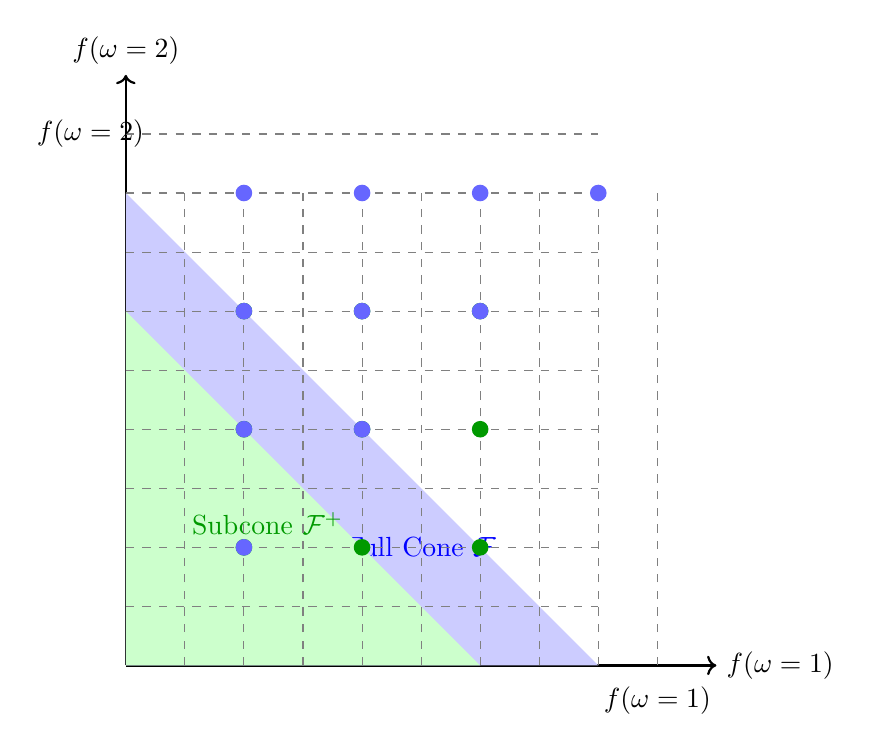
\begin{tikzpicture}[scale=1.5]
        % Axes
        \draw[->, thick] (0, 0) -- (5, 0) node[right] {$f(\omega=1)$};
        \draw[->, thick] (0, 0) -- (0, 5) node[above] {$f(\omega=2)$};
        
        % Full cone
        \fill[blue!20] (0, 0) -- (4, 0) -- (0, 4) -- cycle;
        \node[blue] at (2.5, 1) {Full Cone $\mathcal{F}$};
        
        % Subcone
        \fill[green!20] (0, 0) -- (3, 0) -- (0, 3) -- cycle;
        \node[green!60!black] at (1.2, 1.2) {Subcone $\mathcal{F}^+$};

        % Grid
        \foreach \x in {0.5, 1, 1.5, 2, 2.5, 3, 3.5, 4, 4.5} {
            \draw[dashed, gray] (\x, 0) -- (\x, 4);
            \draw[dashed, gray] (0, \x) -- (4, \x);
        }

        % Points in the subcone
        \foreach \i in {1, 2, 3} {
            \foreach \j in {1, 2, 3} {
                \fill[green!60!black] (\i,\j) circle (2pt);
            }
        }

        % Points in the full cone
        \foreach \i in {1, 2, 3, 4} {
            \foreach \j in {1, 2, 3, 4} {
                \ifnum \i<\j
                    \fill[blue!60] (\i,\j) circle (2pt);
                \else
                    \ifnum \i=\j
                        \fill[blue!60] (\i,\j) circle (2pt);
                    \fi
                \fi
            }
        }

        % Labels
        \node at (4.5, -0.3) {$f(\omega=1)$};
        \node at (-0.3, 4.5) {$f(\omega=2)$};

    \end{tikzpicture}
    \caption{Visualization of the Full Cone $\mathcal{F}$ and the Subcone $\mathcal{F}^+$}
    \label{fig:cone_subcone}
\end{figure}


\dfn{Abstract integral.}{
A function $J:\mathcal{F}\to\mathbb{R}$ is called an abstract integral (on the Stone lattice $\mathcal{F}$) if it has the following three properties:
\begin{enumerate}
    \item Linearity: For $f,g\in\mathcal{F}$ and $\lambda\in\mathbb{R}$,
    \begin{align}
        J(\lambda f)&=\lambda J(f)\\
        J(f+g)&=J(f)+J(g).
    \end{align}
    \item Positive: $J(f)\geq 0$ for all $f\in\mathcal{F}^+$.
    \item Monotone convergence: Let $(f_n)_n$ be a pointwise increasing sequence of functions $f_n\in\mathcal{F}^+$ with limit $f\in\mathcal{F}$. Then,
    \begin{align}
        \lim_{n\to\infty}J(f_n)=J(f).
    \end{align}
\end{enumerate}
}Linearity and positivity of an abstract integral $J$ on $\mathcal{F}$ imply that 
\begin{align*}
    J(f)\leq J(g)\text{ whenever }f,g\in\mathcal{F}\text{ with }f\leq g.
\end{align*}
\ex{}
{    Let $\mathcal{F}$ be the set of all functions (sequences) $f : \mathbb{N} \to \mathbb{R}$ such that $\lim_{\omega \to \infty} f(\omega)$ exists in $\mathbb{R}$. Verify that $\mathcal{F}$ is a Stone lattice. Does $\mathcal{J}(f) := \lim_{\omega \to \infty} f(\omega)$ define an abstract integral on $\mathcal{F}$?}
\begin{myproof}
\begin{enumerate}
    \item Verify that \(\mathcal{F}\) is a Stone Lattice
\begin{itemize}
    \item Lattice Structure:\\
\(\mathcal{F}\) is closed under pointwise addition and scalar multiplication. This means for any \(f, g \in \mathcal{F}\) and \(\alpha \in \mathbb{R}\), \(f + g \in \mathcal{F}\) and \(\alpha f \in \mathcal{F}\).\\
 Pointwise maximum (\(\vee\)) and minimum (\(\wedge\)) of two functions in \(\mathcal{F}\) also belong to \(\mathcal{F}\). For \(f, g \in \mathcal{F}\), define:
     \begin{align*}
       (f \vee g)(\omega) &= \max(f(\omega), g(\omega))\\
     (f \wedge g)(\omega) &= \min(f(\omega), g(\omega))  
     \end{align*}
Both \(\max(f(\omega), g(\omega))\) and \(\min(f(\omega), g(\omega))\) have limits as \(\omega \to \infty\), since the limit of a bounded sequence of real numbers exists.

\item Distributive Property:\\
For all \(f, g, h \in \mathcal{F}\):
     \begin{align*}
     f \vee (g \wedge h) = (f \vee g) \wedge (f \vee h)
     \end{align*}
This follows from the properties of \(\max\) and \(\min\) functions.

\item Pseudocomplement:\\
The pseudocomplement of a function \(f \in \mathcal{F}\) is another function \(g \in \mathcal{F}\) such that \(f \wedge g = 0\) (pointwise zero) and \(f \vee g\) is the smallest function with this property.
\end{itemize}
Therefore, \(\mathcal{F}\) satisfies the requirements to be a Stone lattice.

\item Abstract Integral \(\mathcal{J}(f) := \lim_{\omega \to \infty} f(\omega)\)\\
To determine if \(\mathcal{J}(f) = \lim_{\omega \to \infty} f(\omega)\) defines an abstract integral on \(\mathcal{F}\), we need to check if it satisfies the properties of an integral:
\begin{itemize}
\item Linearity:
For \(f, g \in \mathcal{F}\) and \(\alpha, \beta \in \mathbb{R}\):
     \begin{align*}
     \mathcal{J}(\alpha f + \beta g) = \lim_{\omega \to \infty} (\alpha f(\omega) + \beta g(\omega)) = \alpha \lim_{\omega \to \infty} f(\omega) + \beta \lim_{\omega \to \infty} g(\omega) = \alpha \mathcal{J}(f) + \beta \mathcal{J}(g)
     \end{align*}
This shows that \(\mathcal{J}\) is linear.

\item Monotonicity:\\
If \(f \leq g\) pointwise, then \(\mathcal{J}(f) \leq \mathcal{J}(g)\) because limits preserve the order of sequences:
     \begin{align*}
     \text{If } f(\omega) \leq g(\omega) \text{ for all } \omega, \text{ then } \lim_{\omega \to \infty} f(\omega) \leq \lim_{\omega \to \infty} g(\omega)
     \end{align*}
Therefore, \(\mathcal{J}\) is monotone.

\item Positivity:If \(f \geq 0\) pointwise, then \(\mathcal{J}(f) \geq 0\).
\end{itemize}
Given these properties, \(\mathcal{J}(f) = \lim_{\omega \to \infty} f(\omega)\) defines an abstract integral on \(\mathcal{F}\).
\end{enumerate}
Conclusion:
\(\mathcal{F}\), the set of all functions \(f : \mathbb{N} \to \mathbb{R}\) such that \(\lim_{\omega \to \infty} f(\omega)\) exists, is a Stone lattice. The functional \(\mathcal{J}(f) := \lim_{\omega \to \infty} f(\omega)\) defines an abstract integral on \(\mathcal{F}\).
\end{myproof}
\ex{}
{
Let \(\mathcal{F}\) be the set of all functions (sequences) \(f : \mathbb{N} \to \mathbb{R}\) such that \(\{f \neq 0\}\) is finite. Show that \(\mathcal{F}\) is a Stone lattice, \(\mathcal{F}^* = [0, \infty]^\mathbb{N}\), and \(\mathcal{U}(\mathcal{F}) = \mathcal{P}(\mathbb{N})\).
}
\begin{myproof}
    \begin{enumerate}
        \item Verify that \(\mathcal{F}\) is a Stone Lattice.
        \begin{itemize}
            \item Addition and Scalar Multiplication:\\
            If \(f, g \in \mathcal{F}\), then \(f + g \in \mathcal{F}\) because the sum of two functions that are nonzero on finite sets is also nonzero on a finite set.\\
            If \(\alpha \in \mathbb{R}\), then \(\alpha f \in \mathcal{F}\), provided that \(\alpha \neq 0\).
            \item Pointwise Maximum and Minimum:\\
     For \(f, g \in \mathcal{F}\), \((f \vee g)(n) = \max(f(n), g(n))\) and \((f \wedge g)(n) = \min(f(n), g(n))\).\\
     Both \(\max(f(n), g(n))\) and \(\min(f(n), g(n))\) will be nonzero on finite sets if \(f\) and \(g\) are nonzero on finite sets.
\item Distributive Property:\\
   For all \(f, g, h \in \mathcal{F}\):
     \begin{align*}
         f \vee (g \wedge h) = (f \vee g) \wedge (f \vee h)
     \end{align*}
    
     This holds due to the properties of the maximum and minimum functions.

\item Pseudocomplement:\\
   The pseudocomplement of a function \(f \in \mathcal{F}\) can be considered as a function \(g \in \mathcal{F}\) such that \(f \wedge g = 0\) and \(f \vee g\) is the smallest function with this property.\\

Thus, \(\mathcal{F}\) satisfies the requirements to be a Stone lattice.
        \end{itemize}
        \item Show that \(\mathcal{F}^* = [0, \infty]^\mathbb{N}\)
\(\mathcal{F}^*\) is the dual of \(\mathcal{F}\), representing all functions that are pointwise bounded above by non-negative sequences extending to infinity.\\
\(\mathcal{F}^* = [0, \infty]^\mathbb{N}\) means it includes all functions from \(\mathbb{N}\) to \([0, \infty]\).\\
Given that \(\mathcal{F}\) consists of functions that are zero except for finitely many points, every non-negative sequence in \([0, \infty]^\mathbb{N}\) can be represented in \(\mathcal{F}^*\).
\item Show that \(\mathcal{U}(\mathcal{F}) = \mathcal{P}(\mathbb{N})\)

\(\mathcal{U}(\mathcal{F})\) denotes the ultrafilter generated by \(\mathcal{F}\), which corresponds to the set of all subsets of \(\mathbb{N}\).\\
Since any subset of \(\mathbb{N}\) can be represented as the set where a function in \(\mathcal{F}\) is non-zero, \(\mathcal{U}(\mathcal{F}) = \mathcal{P}(\mathbb{N})\).\\
Every subset of \(\mathbb{N}\) can be generated by the finite non-zero sequences, demonstrating the equality with the power set \(\mathcal{P}(\mathbb{N})\).
    \end{enumerate}
Conclusion:
\begin{itemize}
\item \(\mathcal{F}\) is a Stone lattice.
\item \(\mathcal{F}^* = [0, \infty]^\mathbb{N}\).
\item \(\mathcal{U}(\mathcal{F}) = \mathcal{P}(\mathbb{N})\).
\end{itemize}
\end{myproof}
\ex{}{
Let \(\Omega\) be any uncountable set, and let \(\mathcal{F}\) be the set of all functions \(f : \Omega \to \mathbb{R}\) such that \(\{f \neq 0\}\) is finite. Show that \(\mathcal{F}\) is a Stone lattice, and determine the corresponding sets \(\mathcal{F}^*\), \(\mathcal{U}(\mathcal{F})\), and \(\sigma(\mathcal{F})\).
}
\begin{myproof}
\begin{enumerate}
\item Verify that \(\mathcal{F}\) is a Stone Lattice:
\begin{itemize}
    \item Addition and Scalar Multiplication:\\
If \(f, g \in \mathcal{F}\), then \(f + g \in \mathcal{F}\) because the sum of two functions that are nonzero on finite sets is also nonzero on a finite set.\\
If \(\alpha \in \mathbb{R}\), then \(\alpha f \in \mathcal{F}\), provided that \(\alpha \neq 0\).
\item Pointwise Maximum and Minimum:\\
For \(f, g \in \mathcal{F}\), \((f \vee g)(\omega) = \max(f(\omega), g(\omega))\) and \((f \wedge g)(\omega) = \min(f(\omega), g(\omega))\).\\
Both \(\max(f(\omega), g(\omega))\) and \(\min(f(\omega), g(\omega))\) will be nonzero on finite sets if \(f\) and \(g\) are nonzero on finite sets.
\item Distributive Property:\\
For all \(f, g, h \in \mathcal{F}\):
     \begin{align*}
         f \vee (g \wedge h) = (f \vee g) \wedge (f \vee h)
     \end{align*}
     This holds due to the properties of the maximum and minimum functions.

\item  Pseudocomplement:\\
The pseudocomplement of a function \(f \in \mathcal{F}\) can be considered as a function \(g \in \mathcal{F}\) such that \(f \wedge g = 0\) and \(f \vee g\) is the smallest function with this property.

Thus, \(\mathcal{F}\) satisfies the requirements to be a Stone lattice.
\end{itemize}
\item Determine \(\mathcal{F}^*\)\\

\(\mathcal{F}^*\) represents the set of all functions that are pointwise bounded above by non-negative sequences extending to infinity. Given the context of \(\mathcal{F}\), it represents the dual functions:\\
\(\mathcal{F}^* = [0, \infty]^\Omega\) means it includes all functions from \(\Omega\) to \([0, \infty]\).\\
Since \(\mathcal{F}\) consists of functions that are zero except for finitely many points, every non-negative function in \([0, \infty]^\Omega\) can be represented in \(\mathcal{F}^*\).

\item Determine \(\mathcal{U}(\mathcal{F})\)\\

\(\mathcal{U}(\mathcal{F})\) denotes the ultrafilter generated by \(\mathcal{F}\), which corresponds to the set of all subsets of \(\Omega\).\\
Since any subset of \(\Omega\) can be represented as the set where a function in \(\mathcal{F}\) is non-zero, \(\mathcal{U}(\mathcal{F}) = \mathcal{P}(\Omega)\).\\
Every subset of \(\Omega\) can be generated by the finite non-zero sequences, demonstrating the equality with the power set \(\mathcal{P}(\Omega)\).

\item Determine \(\sigma(\mathcal{F})\)\\
\(\sigma(\mathcal{F})\) refers to the \(\sigma\)-algebra generated by \(\mathcal{F}\).\\
Given \(\mathcal{F}\) consists of functions that are non-zero only on finite sets, \(\sigma(\mathcal{F})\) will include all finite and cofinite subsets of \(\Omega\).\\
A cofinite set is one whose complement is finite, and these sets form a \(\sigma\)-algebra because they are closed under countable unions, intersections, and complements.
\end{enumerate}
Conclusion:
\begin{itemize}
\item \(\mathcal{F}\) is a Stone lattice.
\item \(\mathcal{F}^* = [0, \infty]^\Omega\).
\item \(\mathcal{U}(\mathcal{F}) = \mathcal{P}(\Omega)\).
\item \(\sigma(\mathcal{F})\) is the \(\sigma\)-algebra of all finite and cofinite subsets of \(\Omega\).
\end{itemize}
\end{myproof}
From now on, let $J:\mathcal{F}\to\mathbb{R}$ be an abstract integral. We extend $J$ to a functional on the extension $\mathcal{F}^{\star}$ of $\mathcal{F}^+$. For $g\in\mathcal{F}^{\star}$,let
\begin{align*}
    J(g):=\sup_{f\in\mathcal{F}^+:f\leq g}J(f).
\end{align*}
\nt{
If $g\in\mathcal{F}^+$,then $J(f)\leq J(g)$ for all $f\in\mathcal{F}^+$ such that $f\leq g$,so the new definition $J(g)$ yields the former value of $J(g)$. For $g,h\in\mathcal{F}^{\star}$,
\begin{align*}
    J(g)\leq J(h)\text{ if }g\leq h,
\end{align*}because $g\leq h\Rightarrow\{f:\mathcal{F}^+:f\leq g\}\subset\{f\in\mathcal{F}^+:f\leq g\}$.
}
\mlenma{Representation of $J(g)$}{
If $g=\lim_{n\to\infty}f_n$ with a pointwise increasing sequence $(f_n)_n$ in $\mathcal{F}^+$,then $J(g)=\lim_{n\to\infty}J(f_n)$
.}
\begin{myproof}
    Since $(f_n)_n$ is pointwise increasing,the sequence $(J(f_n))_n$ is increasing,and $f_n\leq g$ for each $n$,whence $J(g)\geq\lim_{n\to\infty}J(f_n)$.\\
    On the other hand,if $f$ is any fixed function on $\mathcal{F}^+$ such that $f\leq g$,then $(f_n\wedge f)_n$ is pointwise increasing with limit $f$. Consequently,
    \begin{align*}
        \lim_{n\to\infty}J(f_n)\geq \lim_{n\to\infty}J(f_n\wedge f)=J(f)\Rightarrow J(g)\leq\lim_{n\to\infty}J(f_n).
    \end{align*}
\end{myproof}
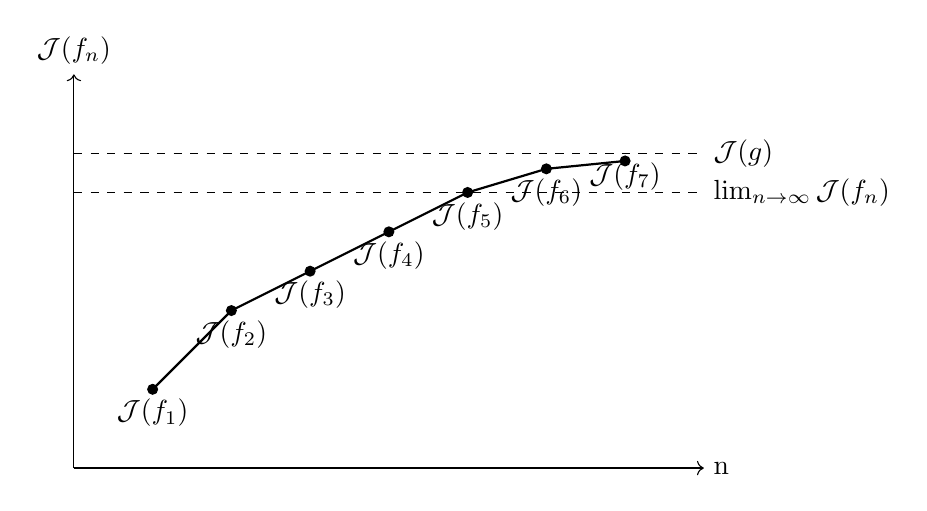
\begin{tikzpicture}
% Axes
\draw[->] (0, 0) -- (8, 0) node[right] {n};
\draw[->] (0, 0) -- (0, 5) node[above] {\(\mathcal{J}(f_n)\)};
% Sequence values
\foreach \x/\y in {1/1, 2/2, 3/2.5, 4/3, 5/3.5, 6/3.8, 7/3.9} {
\fill (\x, \y) circle (2pt);
}
% Limits and bounds
\draw[dashed] (0, 4) -- (8, 4) node[right] {\(\mathcal{J}(g)\)};
\draw[dashed] (0, 3.5) -- (8, 3.5) node[right] {\(\lim_{n \to \infty} \mathcal{J}(f_n)\)};
% Sequence line
\draw[thick] (1, 1) -- (2, 2) -- (3, 2.5) -- (4, 3) -- (5, 3.5) -- (6, 3.8) -- (7, 3.9);
% Labels
\node at (1, 0.7) {\(\mathcal{J}(f_1)\)};
\node at (2, 1.7) {\(\mathcal{J}(f_2)\)};
\node at (3, 2.2) {\(\mathcal{J}(f_3)\)};
\node at (4, 2.7) {\(\mathcal{J}(f_4)\)};
\node at (5, 3.2) {\(\mathcal{J}(f_5)\)};
\node at (6, 3.5) {\(\mathcal{J}(f_6)\)};
\node at (7, 3.7) {\(\mathcal{J}(f_7)\)};
\end{tikzpicture}
\mlenma{}{
For arbitrary $c\geq 0$ and functions $g,g_1,g_2,\cdots\in\mathcal{F}^{\star}$,
\begin{align}
    J(cg)&=cJ(g)\\
    J(\sum_{n\geq 1}g_n)&=\sum_{n\geq 1}J(g_n)
\end{align}If $(g_n)_{n\geq 1}$ is pointwise increasing with limit $g$,then
\begin{align}
    J(g)=\lim_{n\to\infty}J(g_n).
\end{align}
}
This lemma shows that $J$ as a functional on $\mathcal{F}^{\star}$ has the desirable properties.
\thm{Daniell-Port-Stone.}{
There exists a unique measure $\mu$ on the $\sigma-$algebra $\sigma(\mathcal{F})$ with the following properties:$\mathcal{F}\subset\mathcal{L}^1(\mu)$,
\begin{align}
    J(f)=\int f\,d\mu\text{ for all }f\in\mathcal{F},
\end{align}and for any set $B\in\sigma(\mathcal{F})$,
\begin{align}
    \mu(B)=\inf\{\mu(U):U\in\mathcal{U}(\mathcal{F}),U\supset B\}
\end{align}with $\inf(\emptyset):=\infty$.
}
\section{Representations of Dual Spaces}
Suppose that $\mathcal{F}$ is an arbitrary real vector space,equipped with a seminorm $\|\cdot\|$. 
\nt{
\begin{enumerate}
    \item The \textcolor{blue}{dual space of $(\mathcal{F},\|\cdot\|)$} is the space of linear functionals $L:\mathcal{F}\to\mathbb{R}$ which are continuous w.r.t.the seminorm $\|\cdot\|$.
    \item \textcolor{blue}{Continuity of $L$}:$\sup_{f\in\mathcal{F},\|f\|\leq 1}|L(f)|<\infty$.
\end{enumerate}
}
\qs{}{How can the dual space be represented explicitly?}
Let $\mathcal{F}$ be a Stone lattice of functions on a set $\Omega$. Suppose that there is a seminorm $\|\cdot\|$ on $\mathcal{F}$ satisfying the following two properties:
\begin{enumerate}
    \item $\|f\|\leq\|g\|\text{ whenever }f,g\in\mathcal{F}^+\text{ with }f\leq g$.
    \item For any pointwise decreasing sequence $(f_n)_{n\geq 1}$ in $\mathcal{F}^+$ with limit $0$,
    \begin{align*}
        \lim_{n\to\infty}\|f_n\|=0.
    \end{align*}
\end{enumerate} 
\thm{Any continuous linear functional on $(\mathcal{F},\|\cdot\|)$ can be represented with certain integrals.}{
For any functional $L$ in the dual space of $(\mathcal{F},\|\cdot\|)$ there exist measures $\mu^+,\mu^-$ on $\sigma(\mathcal{F})$ such that $\mathcal{F}\subset\mathcal{L}^1(\mu^++\mu^-)$ and
\begin{align}
    L(f)=\int f\,d\mu^+-\int f\,d\mu^-\text {for all }f\in\mathcal{F}.
\end{align}
}
\begin{tcolorbox}[colback=orange!10!white, colframe=orange!50!black, title=Theorem 2.18]
    For any functional \( L \) in the dual space of \((\mathcal{F}, \|\cdot\|)\), there exist measures \( \mu^+ \) and \( \mu^- \) on \( \sigma(\mathcal{F}) \) such that:
    \[
    \mathcal{F} \subset L^1(\mu^+ + \mu^-)
    \]
    and
    \[
    L(f) = \int f \, d\mu^+ - \int f \, d\mu^- \quad \text{for all } f \in \mathcal{F}.
    \]
\end{tcolorbox}

\begin{figure}[ht]
    \centering
    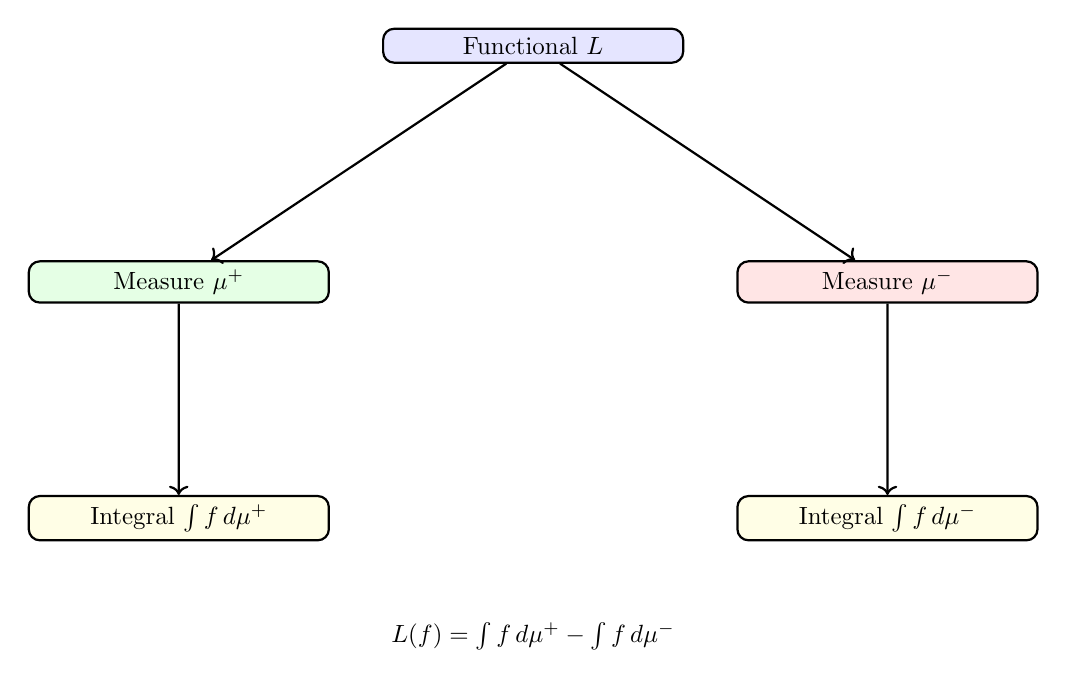
\begin{tikzpicture}[scale=1.5, every node/.style={scale=0.9}]
        % Functional L
        \node[draw, thick, rounded corners, fill=blue!10, text width=4cm, align=center] (L) at (0, 4) {Functional $L$};
        
        % Measures
        \node[draw, thick, rounded corners, fill=green!10, text width=4cm, align=center] (mu_plus) at (-3, 2) {Measure $\mu^+$};
        \node[draw, thick, rounded corners, fill=red!10, text width=4cm, align=center] (mu_minus) at (3, 2) {Measure $\mu^-$};
        
        % Integrals
        \node[draw, thick, rounded corners, fill=yellow!10, text width=4cm, align=center] (int_plus) at (-3, 0) {Integral $\int f \, d\mu^+$};
        \node[draw, thick, rounded corners, fill=yellow!10, text width=4cm, align=center] (int_minus) at (3, 0) {Integral $\int f \, d\mu^-$};
        
        % Arrows
        \draw[->, thick] (L) -- (mu_plus);
        \draw[->, thick] (L) -- (mu_minus);
        \draw[->, thick] (mu_plus) -- (int_plus);
        \draw[->, thick] (mu_minus) -- (int_minus);
        
        % Final equation
        \node at (0, -1) {$L(f) = \int f \, d\mu^+ - \int f \, d\mu^-$};
    \end{tikzpicture}
    \caption{Visualization of Theorem 2.18: Decomposition of a functional \( L \) in the dual space into integrals with respect to measures \( \mu^+ \) and \( \mu^- \).}
    \label{fig:theorem_2_18}
\end{figure}


\mlenma{From additive,nonnegative to linear functionals.}{
Suppose that $J:\mathcal{F}^+\to [0,\infty)$ is a functional which is additive in the sense that $J(f+g)=J(f)+J(g)$ for all $f,g\in\mathcal{F}^+$. Then,
\begin{align}
    L(f):=J(f^+)-J(f^-)
\end{align}defines a linear functional $L:\mathcal{F}\to\mathbb{R}$ such that $L=J$ on $\mathcal{F}^+$.
}
\mlenma{From linear to additive,nonnegative functionals}{
Suppose that $L:\mathcal{F}\to\mathbb{R}$ is a linear functional. For $f\in\mathcal{F}^+$ let
\begin{align}
    J(f):&=\sup\{L(h):h\in\mathcal{F}^+,h\leq f\}\\
    K(f):&=\sup\{-L(h):h\in\mathcal{F}^+,h\leq f\}。
\end{align}These two functionals $J,K:\mathcal{F}^+\to[0,\infty]$ are additive in the sense that $J(f+g)=J(f)+J(g)$ and $K(f+g)=K(f)+K(g)$ for all $f,g\in\mathcal{F}^+$.\\
They satisfy the equations $J=K+L$ and $K=J-L$ on $\mathcal{F}^+$. In particular, $J$ is real-valued iff $K$ is real-valued.\\
If $J$ and $K$ are real-valued,then for arbitrary $f\in\mathcal{F}$,
\begin{align}
    L(f)=L_J(f)-L_K(f),
\end{align}where $L_J(f):=J(f^+)-J(f^-)$ and $L_K(f):=K(f^+)-K(f^-)$
}
\begin{figure}[ht]
    \centering
    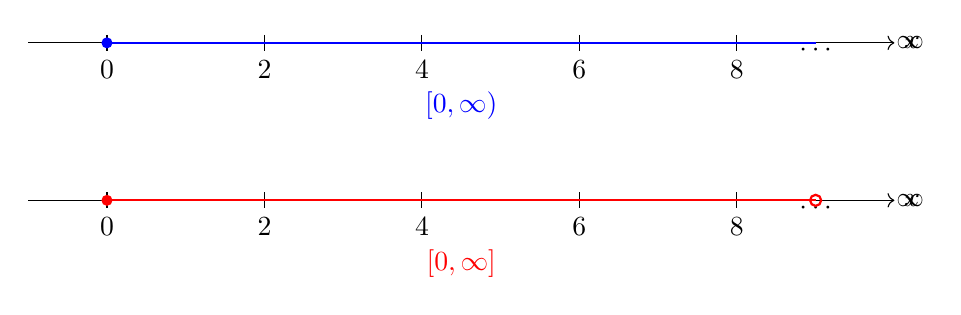
\begin{tikzpicture}
        % Draw number line
        \draw[->] (-1,0) -- (10,0) node[right] {$x$};

        % Label the points
        \foreach \x in {0, 2, 4, 6, 8} {
            \draw (\x,0.1) -- (\x,-0.1) node[below] {\x};
        }
        \node at (9, -0.1) {\(\cdots\)};

        % Interval [0, infinity)
        \draw[thick, blue] (0,0) -- (9,0);
        \fill[blue] (0,0) circle (2pt);
        \node[blue, below] at (4.5, -0.5) {$[0, \infty)$};

        % Draw number line
        \draw[->] (-1,-2) -- (10,-2) node[right] {$x$};

        % Label the points
        \foreach \x in {0, 2, 4, 6, 8} {
            \draw (\x,-1.9) -- (\x,-2.1) node[below] {\x};
        }
        \node at (9, -2.1) {\(\cdots\)};

        % Interval [0, infinity]
        \draw[thick, red] (0,-2) -- (9,-2);
        \fill[red] (0,-2) circle (2pt);
        \draw[red, thick] (9,-2) circle (2pt);
        \node[red, below] at (4.5, -2.5) {$[0, \infty]$};

        % Infinity symbol
        \node at (10.2, 0) {$\infty$};
        \node at (10.2, -2) {$\infty$};

    \end{tikzpicture}
    \caption{Visual comparison of the intervals \([0, \infty)\) and \([0, \infty]\).}
    \label{fig:intervals}
\end{figure}\\

\textcolor{red}{One application is about continuous functions on compact metric spaces}.
\thm{Riesz-Markov-Kakutani}{
Let $(\Omega,d)$ be a compact metric space and let $\mathcal{C}(\Omega)$ be the family of continuous functions $f:\Omega\to\mathbb{R}$ w.r.t. $d$,equipped with the supremum norm $\|\cdot\|_{\infty}$,that is,$\|f\|_{\infty}=\max_{\omega\in\Omega}|f(\omega)|$. Let $L:\mathcal{C}(\Omega)\to\mathbb{R}$ be a linear functional which is continuous w.r.t.$\|\cdot\|_{\infty}$. Then there exists a \textcolor{red}{finite signed measure $\nu$} on $\text{Borel}(\Omega)$ such that 
\begin{align}
    L(f)=\int f\,d\nu=\int f\,d\mu^+-\int f\,d\mu^-,\text{ for all }f\in\mathcal{C}(\Omega),
\end{align}where $\nu=\mu^+-\mu^-$ with finite measures $\mu^+,\mu^-$ on $\text{Borel}(\Omega)$.
}
\textcolor{red}{The conclusion can be reformulated as follows:There exists a probability measure $P$ on $\text{Borel}(\Omega)$ and a bounded,measurable function $h:\Omega\to\mathbb{R}$ such that
\begin{align}
    L(f)=\int fh\,dP\text{ for all }f\in\mathcal{C}(\Omega).
\end{align}}
\mlenma{Dini}{
Let $(\Omega,d)$ be a compact metric space,and let $(f_n)_{n\geq 1}$
 be a pointwise decreasing sequence of continuous functions with limit $0$. Then $\|f_n-f\|_{\infty}\to 0$ as $n\to\infty$.
 }
 Let $(\Omega,\SA,\mu)$ be a $\sigma-$finite measure space. For $p\in[1,\infty)$ let $\mathcal{L}^p(\mu)$ be the set of measurable functions $f:\Omega\to\mathbb{R}$ such that 
 \begin{align}
     \|f\|_{p,\mu}:=(\int|f|^p\,d\mu)^{\frac{1}{p}}<\infty.
 \end{align}$\mathcal{L}^p(\mu)$ is a Stone Lattice and $\|\cdot\|_{p,\mu}$ defines a seminorm on $\mathcal{L}^p(\mu)$. \\
 \textcolor{red}{The set $\mathcal{L}^{\infty}(\mu)$ of measurable functions $f:\Omega\to\mathbb{R}$ such that
 \begin{align}
     \|f\|_{\infty,\mu}:=\inf\{r\geq 0:\mu(\{|f|>r\})=0\}<\infty.
 \end{align}}
 \thm{}{
 For an arbitrary $p\in[1,\infty)$,let $L:\mathcal{L}^p(\mu)\to\mathbb{R}$ be a linear and continuous w.r.t.$\|\cdot\|_{p,\mu}$. Then there exists an function $h\in\mathcal{L}^q(\mu)$,where $q=\frac{p}{p-1}\in(1,\infty]$,such that
 \begin{align}
     &L(f)=\int fh\,d\mu\text{ for all }f\in\mathcal{L}^p(\mu),\\
     &\sup_{f\in\mathcal{L}^p(\mu),\|f\|_{p,\mu}\leq 1}|L(f)|=\|h\|_{q,\mu}.
 \end{align}The function $h$ is unique $\mu-$almost everywhere.
 }
 \mlenma{Hölder}{
 Let $p\in[1,\infty)$ and $q=\frac{p}{p-1}\in(1,\infty]$. For any function $h\in\mathcal{L}^q(\mu)$,
 \begin{align}
     \sup_{f\in\mathcal{L}^p(\mu),\|f\|_{p,\mu}\leq 1}|\int fh\,d\mu|=\|h\|_{q,\mu}.
 \end{align}
 }
\section{Prohorov's Theorem}
Let $(\Omega,d)$ be a metric space and let $\SA$ be the corresponding Borel-$\sigma-$algebra,that is,the smallest $\sigma-$algebra containing all open and closed subsets of $\Omega$.
\thm{Portmanteau}{
Let $P$ and $P_1,P_2,\cdots$ be probability measures on $\Omega$. The following four statements are equivalent:
\begin{enumerate}
    \item For any $f\in\mathcal{C}_b(\Omega)$,
    \begin{align}
        \lim_{n\to\infty}\int f\,dP_n=\int f\,dP.
    \end{align}
    \item  For any $f\in\mathcal{C}_{Lip,b}(\Omega)$,
    \begin{align}
        \lim_{n\to\infty}\int f\,dP_n=\int f\,dP.
    \end{align}
    \item For any open set $U\subset\Omega$,
    \begin{align}
        \liminf_{n\to\infty}P_n(U)\geq P(U).
    \end{align}
    \item For any closed set $A\subset\Omega$,
    \begin{align}
        \liminf_{n\to\infty}P_n(A)\leq P(A).
    \end{align}
    \item For any Borel set $B\subset\Omega$ with $P(\partial B)=0$,
    \begin{align}
        \lim_{n\to\infty}P_n(B)=P(B).
    \end{align}
\end{enumerate}
}
\dfn{Weak convergence.}{
A sequence $(P_n)_n$ of probability measures on $\Omega$ converges weakly to a probability measure $P$ on $\Omega$ if one condition of Portmanteau-theorem are satisfied.
}
Consider a family $\mathcal{P}$ of probability distributions on $\Omega$.
\qs{}{
Under which condition $\mathcal{P}$,every sequence in $\mathcal{P}$ has a weakly convergent subsequence.
}
\thm{Prohorov.}{
Let $(\Omega,d)$ be complete and separable. The following two properties of $\mathcal{P}$ are equivalent:
\begin{enumerate}
    \item For any fixed $\epsilon>0$,there exists a compact set $K\subset \Omega$ such that
    \begin{align}
        \inf_{P\in\mathcal{P}}P(\Omega\backslash K)\leq\epsilon.
    \end{align}
    \item For any sequence in $\mathcal{P}$,there exists a subsequence converging weakly to some probability distribution on $\Omega$.
\end{enumerate}
}
\nt{
Property(1) is \textcolor{blue}{"tightness of $\mathcal{P}$"}.\\
Since a singleton $\mathcal{P}=\{P\}$ has obviously property(2),we see that any probability distribution is "tight" in the sense that for any $\epsilon>0$ there exists a compact set $K\subset\Omega$ such that $P(\Omega\backslash K)\leq\epsilon$.
}
\mlenma{Separability of $\mathcal{C}(\Omega)$.}{
Let $(\Omega,d)$ be a compact metric space. The Banach space $(\mathcal{C}(\Omega),\|\cdot\|_{\infty})$ is separable.
}
\mlenma{}{
For each $m\in\mathbb{N}$ let $(x_{m,n})_n$ be a bounded sequence of real numbers. Then there exist natural numbers $n(1)<n(2)<n(3)<\cdots$ such that 
\begin{align}
    y_m:=\lim_{s\to\infty}x_{m,n(s)}
\end{align}exists for any $m\in\mathbb{N}$.
}
\section{Summary}
\chapter{Conditional Expectations}
Suppose $(\Omega,\SA,P)$ be a probability space and $X$ be a random variable in $\mathcal{L}^1(P)$.\\
\textcolor{red}{I.e.$X:\Omega\to\mathbb{R}$ is $\SA-$measurable,and $\int|X|\,dP<\infty$.}
\section{Conditional expectations w.r.t. a sub-$\sigma$-algebra}
Suppose $\SA_0$ be a sub-$\sigma-$algebra of $\SA$. Consider a complex random experiment described by $(\Omega,\SA,P)$ and the sub-$\sigma-$algebra $\SA_0$ represents some partial aspects of it.\textcolor{blue}{If the random experiment yields some $\omega\in\Omega$,then the $\sigma-$algebras $\SA$ and $\SA_0$ define the available queries about $\omega$. For each $A\in\SA$ or only for each $A\in\SA_0$ we know whether $\omega$ lies in $A$ or not.} 
\ex{}{
Consider $\SA_0:=\sigma(T)$,where $T(\Omega,\SA)\to(\tau,\mathcal{B})$ is a measurable mapping and $\sigma(T):=\{T^{-1}(B):B\in\mathcal{B}\}$.
}
\thm{}{
There exits a random variable $X_0\in\mathcal{L}^1(P|_{\mathcal{A}_0})$ such that
\begin{align}
    \int_{A_0}X_0\,dP=\int_{A_0}X\,dP\text{ for all }A_0\in\mathcal{A}_0.
\end{align}
This random variable $X_0$ is almost everywhere unique:If $\Tilde{X_0}$ is another random variable satisfying (3.1),then $P(\Tilde{X}_0\neq X_0)=0$.
}
\begin{myproof}
    
\end{myproof}
\dfn{Conditional expectation I.}{
A random variable $X_0$ as in the Theorem 3.1 is called a version of the conditional expectation of $X$,given the sub$-\sigma-$algebra $\SA_0$. A function $X_0$ satisfying $(3.1)$ is denoted by $\mathbb{E}(X|\SA_0)$.
}
If a random variable $X\in\mathcal{L}^1(P)$ is $\SA_0-$measurable,then $\mathbb{E}(X|\SA_0)=X$ almost surely. If $X=c$ almost surely for some constant $c\in\mathbb{R}$,then $\mathbb{E}(X|\SA_0)=c$ almost surely.
\ex{Countable partitions.}{
Let $\Omega=\cup_{n\geq 1}B_n$ with a sequence $(B_n)_{n\geq 1}$ of disjoint measurable sets and let $\SA_0$ be the smallest $\sigma-$algebra containing all these sets $B_n,n\geq 1$. Then 
\begin{align}
    \mathbb{E}(X|\SA_0)=\sum_{n\geq 1}\mathbb{E}(X|B_n)1_{B_n}\text{ almost surely }
\end{align}with the numbers
\begin{align}
    \mathbb{E}(X|B):=\begin{cases}
P(B)^{-1}\int_X\,dP&\text{ if }P(B)>0,\\
\mathbb{E}(X)&\text{ else }.
    \end{cases}
\end{align}
The function $X_0:=\sum_{n\geq 1}\mathbb{E}(X|B_n)1_{B_n}=c$ on each set $B_n,n\geq 1$,so it is $\SA_0-$measurable. Moreover,any set $A_0=\cup_{n_M}B_n\in\SA_0$ with $M\subset\mathbb{N}$,so
\begin{align}
    \int_{A_0}X\,dP&=\sum_{n\in M}\int_{B_n}X\,dP\\
    &=\sum_{n\in M}P(B_n)\mathbb{E}(X|B_n)\\
    &=\sum_{n\in M}\int_{B_n}X_0\,dP\\
    &=\int_{A_0}X_0\,dP.
\end{align}
}
\cor{Properties of conditional expectations.}{
Suppose $X,Y\in\mathcal{L}^1(P)$.
\begin{enumerate}
    \item \textcolor{blue}{linearity of integrals}:For real numbers $a,b$,
    \begin{align}
        \mathbb{E}(aX+bY|\mathcal{A}_0)=a\mathbb{E}(X|\SA_0)+b\mathbb{E}(Y|\SA_0)\text{ almost surely }.
    \end{align}
    \item If $X\leq Y$ almost surely,then
    \begin{align}
        \mathbb{E}(X|\SA_0)\leq\mathbb{E}(Y|\SA_0)\text{ almost surely}.
    \end{align}It follows from $X\leq Y$ almost surely that 
    \begin{align*}
        \int_{A_0}\mathbb{E}(X|\SA_0)\,dP&=\int_{A_0}X\,dP\\
        &\leq \int_{A_0}Y\,dP\\
        &=\int_{A_0}\mathbb{E}(Y|\SA_0)\,dP\text{ for all }A_0\in\SA_0.
    \end{align*}Hence,$P(\mathbb{E}(X|\SA_0)>\mathbb{E}(Y|\SA_0))=0$.
    \item The mapping $X\mapsto\mathbb{E}(X|\SA_0)$ is a weak contraction in the sense that
    \begin{align}
        |\mathbb{E}(X|\SA_0)|\leq \mathbb{E}(|X||\SA_0)\text{ almost surely}.
    \end{align}
    \item \begin{align}
        \int|\mathbb{E}(X|\SA_0)-\mathbb{E}(Y|\SA_0)|\,dP\leq \int|X-Y|\,dP.
    \end{align}
    \item For any $\SA_0-$measurable random variable $Z_0:\Omega\to\mathbb{R}$,
    \begin{align}
        \int XZ_0\,dP=\int\mathbb{E}(X|\SA_0)Z_0\,dP,
    \end{align}whenever the integral is well-defined in $\bar{\mathbb{R}}$.
\end{enumerate}
}
\begin{myproof}
    (3).Suppose $X=X^+-X^-$ with $X^{\pm}=max(\pm X,0)$,then $|X|=X^++X^-$ almost everywhere.
    \begin{align*}
        \mathbb{E}(X^{\pm}|\SA_0)&\geq 0\\
        \mathbb{E}(X|\SA_0)&=\mathbb{E}(X^+-X^-|\SA_0)=\mathbb{E}(X^+|\SA_0)-\mathbb{E}(X^-|\SA_0)\\
        \mathbb{E}(|X||\SA_0)&=\mathbb{E}(X^++X^-|\SA_0)=\mathbb{E}(X^+|\SA_0)+\mathbb{E}(X^_|\SA_0)\\
        \Rightarrow&|\mathbb{E}(X|\SA_0)|\leq\mathbb{E}(|X||\SA_0).
    \end{align*}
\end{myproof}
\ex{}{
Let $P$ be the exponential distribution on $\Omega=[0,\infty)$ with rate parameter $\lambda>0$,and let $\SA_0$ be the smallest $\sigma-$algebra containing all intervals $[k,k+1),k\in\mathbb{N}_0$. Determine $\mathbb{E}(X|\SA_0)$ in case of $X(\omega):=\omega$.
}
\begin{myproof}
    
\end{myproof}
\ex{"Tower property" of conditional expectations.}{
Let $(\Omega,\SA,P)$ be a probability space and $X\in\mathcal{L}^1(P)$. Let $\SA_1$ and $\SA_2$ be $\sigma-$algebras over $\Omega$ such that $\SA_1\subset\SA_2\SA$.
\begin{enumerate}
    \item Show that $\mathbb{E}(\mathbb{E}(X\SA_1)|\SA_2)=\mathbb{E}(X|\SA_1)$ almost surely.
    \item Show that tower property: $\mathbb{E}(\mathbb{E}(X|\SA_2)|\SA_1)=\mathbb{E}(X|\SA_1)$ almost surely.
\end{enumerate}
}
\begin{myproof}
    

\end{myproof}
\mlenma{Extension of Jensen's inequality for expectations to conditional expectations.}{
Let $X\in\mathcal{L}^1(P)$,and let $\psi:\mathbb{R}\to\mathbb{R}$ be convex such that $\int\psi(X)\,dP<\infty$. Then
\begin{align}
    \psi(\mathbb{E}(X|\SA_0))&\leq\mathbb{E}(\psi(X)|\SA_0)\text{ almost surely},\\
    \int\psi(\mathbb{E}(X|\SA_0))\,dP&\leq\int\psi(X)\,dP.
\end{align}
}
\begin{myproof}
    By the definition of conditional expectations,it suffices to show that for any fixed $A_0\in\SA_0$,
    \begin{align*}
        \int_{A_0}\psi(\mathbb{E}(X|\SA_0))\,dP\leq\int_{A_0}\mathbb{E}(\psi(X)|\SA_0)\,dP=\int_{A_0}\psi(X)\,dP.
    \end{align*}
    By the convexity of $\psi$,for any fixed $x_0\in\mathbb{R}$ there exists a slope $b(x_0)\in\mathbb{R}$ such that $\psi(x)\geq\psi(x_0)+b(x_0)(x-x_0)$ for all $x\in\mathbb{R}$.\\
    For arbitrary $x\in\mathbb{R}$,
    \begin{align*}
        \psi(x)=\sup_{x_0\in\mathbb{Q}}(\psi(x_0)+b(x_0)(x-x_0)),
    \end{align*}because $\psi$ is continuous and $b(\cdot)$ non-decreasing. Consequently,
    \begin{align*}
        \int_{A_0}\psi(\mathbb{E}(X|\SA_0))\,dP&=\int_{A_0}\sup_{x_0\in\mathbb{Q}}(\psi(x_0)+b(x_0)(\mathbb{E}(X|\SA_0)-x_0))\,dP\\
        &=\int_{A_0}\sup_{x_0\in\mathbb{Q}}\mathbb{E}(\psi(x_0)+b(x_0)(X-x_0)|\SA_0)\,dP\\
        &\leq\int_{A_0}\mathbb{E}(\psi(X)|\SA_0)\,dP.
    \end{align*}Use countability of $\mathbb{Q}$ to conclude that
    \begin{align*}
        \psi(x_0)+b(x_0)(\mathbb{E}(X|\SA_0)-x_0)&=\mathbb{E}(\psi(x_0)+b(x_0)(X-x_0)|\SA_0)\\
        &\leq \mathbb{E}(\psi(X)|\SA_0)
    \end{align*}simultaneously for all $x_0\in\mathbb{Q}$ almost surely.
\end{myproof}
\section{Conditional expectations as orthogonal projections}
Restrict our attention to the space $\mathcal{L}^2(P)\subset\mathcal{L}^1(P)$ of square-integrable random variables. If we identify random variables which are equal almost surely, we obtain the Hilbert space $\mathcal{L}^2(P)$ with inner product 
\begin{align}
    <X,Y>:=\int XY\,dP.
\end{align}and norm
\begin{align}
    \|X\|:=<X,X>^{\frac{1}{2}}=(\int X^2\\,dP)^{\frac{1}{2}}.
\end{align}
\nt{
One may view $\mathbb{E}(\cdot|_{\SA_0})$ as a continuous linear mapping from $\mathcal{L}^2(P)$ to its closed linear subspace $\mathcal{L}^2(P_{\SA_0})$. Apply Jensen's inequality with $\psi(x):=x^2$ leads to the inequality
\begin{align*}
    \int \mathbb{E}(X|\SA_0)^2\,dP\leq \int X^2\,dP.
\end{align*}
}
\thm{}{
The mapping $X\mapsto\mathbb{E}(X|_{\SA_0})$ is the orthogonal linear projection of $\mathcal{L}^2(P)$ onto $\mathcal{L}^2(P|_{\SA_0})$. Precisely,for arbitrary random variables $X\in\mathcal{L}^2(P)$ and $Y_0\in\mathcal{L}^2(P|_{\SA_0})$,
\begin{align}
    \|X-Y_0\|^2&=\|X-\mathbb{E}(X|\SA_0)\|^2+\|\mathbb{E}(X|\SA_0)-Y_0\|^2\\
    &\geq \|X-\mathbb{E}(X|\SA_0)\|^2
\end{align}with equality if and only if $Y_0=\mathbb{E}(X|\SA_0)$. In particular,
\begin{align}
    \|X\|^2=\|X-\mathbb{E}(X|\SA_0)\|^2+\|\mathbb{E}(X|\SA_0)\|^2\geq\|\mathbb{E}(X|\SA_0)\|^2
\end{align}with equality iff $X=\mathbb{E}(X|\SA_0)$.
}
\nt{
\begin{align}
    \mathbb{E}(\mathbb{E}(X|\SA_0))&=\int_{\Omega}\mathbb{E}(X|\SA_0)\,dP=\int_{\Omega}X\,dP=\mathbb{E}(X)\\
    \|X-\mathbb{E}(X|\SA_0)\|^2&=Var(X)-Var(\mathbb{E}(X|\SA_0)).
\end{align}
}
\begin{myproof}
    Suppose $X_0:=\mathbb{E}(X|\SA_0)$,by $<X,Y_0>=\int XY_0\,dP=\int X_0Y_0\,dP=<X_0,Y_0>$,whence
    \begin{align*}
        \|X-Y_0\|^2&=\|X\|^2-2<X,Y_0>+\|Y_0\|^2\\
        &=\|X\|^2-2<X_0,Y_0>+\|Y_0\|^2\\
        &=\|X\|^2-\|X_0\|^2+\|X_0\|^2-2<X_0,Y_0>+\|Y_0\|^2\\
        &=\|X\|^2-\|X_0\|^2+\|X_0-Y_0\|^2\\
        &\geq \|X\|^2-\|X_0\|^2
    \end{align*}with equality if and only if $Y_0=X_0$. In particular,setting $Y_0=X_0$ shows that $\|X-X_0\|^2=\|X\|^2-\|X_0\|^2$,which is equivalent to the second asserted equation $\|X\|^2=\|X-X_0\|^2+\|X_0\|^2$,and we obtain the general equality
    \begin{align*}
        \|X-Y_0\|^2=\|X-X_0\|^2+\|X_0-Y_0\|^2.
    \end{align*}
\end{myproof}
\ex{}{
Let $P$ be the exponential distribution on $\Omega=[0,\infty)$ with rate parameter $\lambda>0$,let $\SA_0$ be the smallest $\sigma-$algebra containing all intervals $[k,k+1),k\in\mathbb{N}_0$,and let $X(\omega):=\omega$. Determine the value of 
\begin{align*}
    \|X-\mathbb{E}(X|\SA)\|.
\end{align*}
HINTS:$\mathbb{E}(X|\SA_0)=Y+\mathbb(X)-\mathbb{E}(Y)$,where $Y\sim \text{Geom}(p)$ with $p=1-e^{-\lambda}$.
}
\section{Conditional expectations given another random variable}
Suppose that instead of the random outcome $\omega\in\Omega$ we only know $T(\omega)$ for some given measurable function $T:(\Omega,\SA)\to(\tau,\mathcal{B})$. This corresponds to the sub$-\sigma-$algebra
\begin{align}
    \sigma(T):=\{T^{-1}(B):B\in\mathcal{B}\}
\end{align}of $\mathcal{A}$. It is the smallest $\sigma-$algebra $\SA_0$ over $\Omega$ such that $T$ is $\SA_0-\mathcal{B}-$measurable. There is a simple result about $\sigma(T)-$measuable functions $X:\Omega\to\mathbb{R}$.
\thm{Lifting.}{
A mapping $X:\Omega\to\mathbb{R}$ is $\sigma(T)-$measurable if and only if
\begin{align}
    X=V\circ T
\end{align}for some $\mathcal{B}-$measurable function $V:\tau\to\mathbb{R}$.
}\textcolor{red}{$V\circ T$ stands for the mapping $\Omega\ni\omega\mapsto V(T(\omega))\in\mathbb{R}$.}
\nt{
Elementary result: the probability measure 
\begin{align*}
    \mathcal{B}\ni B\mapsto P^T(B):=P(T\in B).
\end{align*}
}
\ex{Change of variables.}{
Show that for any real-valued random variable $V$ on the probability space $(\tau,\mathcal{B},P^T)$ and any set $B\in\mathcal{B}$,
\begin{align*}
    \int_{T^{-1}(B)}V(T)\,dP=\int_BV\,dP^T,
\end{align*}provided that one of these two integrals is well-defined in $\bar{\mathbb{R}}$.\\
HINT: Use approximations of $V$.
}
\thm{}{
For any random variable $X\in\mathcal{L}^1(P)$ there exists a random variable $V\in\mathcal{L}^1(P^T)$ such that
\begin{align}
    \int_{T^{-1}(B)}X\,dP=\int_B V\,dP^T \text{for arbitrary }B\in\mathcal{B}.
\end{align}
}This random variable $V$ is almost everywhere unique in the following sense: If $\Tilde{V}$ is another random variable then $P^T(\Tilde{V}\neq V)=0$.
\dfn{Conditional expectation,2.}{
A random variable $V$ as in Theorem 3.3.2 is called a version of the conditional expectation of $X$,given the random variable $T$. For any such random variable $V$ we write $\mathbb{E}(X|T)$ instead of $V$ and $\mathbb{E}(X|T=t)$ instead of$\mathbb{E}(V|T=t)$ instead of $\mathbb{E}(V|T)(t)$.
}
\textcolor{red}{$\mathbb{E}(X|T)$}
\section{Summary}

\chapter{Stochastic Kernels}

\section{Stochastic Kernels and Fubini's Theorem}

\section{Decomposing Measures on Product Spaces}

\section{Conditional Expectations and Distributions}

\section{Summary}

\end{document}
